% Whole-tumour patient-similarity graph manuscript, formatted for the Arabian Journal for Science and Engineering (AJSE).
% Springer Nature LaTeX template (sn-jnl.cls), two-column option [iicol] as requested in the AJSE author guidelines,
% numbered references in square brackets (sn-nature.bst with natbib "numbers").
% Every number in the text comes from tables/numbers.tex.

\PassOptionsToPackage{table}{xcolor}
\documentclass[pdflatex,iicol,sn-nature]{sn-jnl}

\usepackage{graphicx}
\usepackage{amsmath,amssymb,amsfonts}
\usepackage{xcolor}
\usepackage{textcomp}
\usepackage{booktabs}
\usepackage{tabularx}
\usepackage{array}
\usepackage{multirow}
\usepackage{tikz}
\usetikzlibrary{arrows.meta,positioning,calc,fit,backgrounds,shapes.geometric}

\graphicspath{{figures/}}
\newcommand{\ablPrimBurDMMax}{0.84}
\newcommand{\ablPrimBurDMMin}{0.65}
\newcommand{\ablPrimBurLRMax}{0.63}
\newcommand{\ablPrimBurLRMin}{0.58}
\newcommand{\ablPrimBurOSMax}{0.69}
\newcommand{\ablPrimBurOSMin}{0.65}
\newcommand{\ablPrimVolDMMax}{0.78}
\newcommand{\ablPrimVolDMMin}{0.65}
\newcommand{\ablPrimVolLRMax}{0.63}
\newcommand{\ablPrimVolLRMin}{0.58}
\newcommand{\ablPrimVolOSMax}{0.70}
\newcommand{\ablPrimVolOSMin}{0.65}
\newcommand{\ablTotBurDMMax}{0.87}
\newcommand{\ablTotBurDMMin}{0.85}
\newcommand{\ablTotBurLRMax}{0.63}
\newcommand{\ablTotBurLRMin}{0.59}
\newcommand{\ablTotBurOSMax}{0.73}
\newcommand{\ablTotBurOSMin}{0.70}
\newcommand{\ablTotVolDMMax}{0.88}
\newcommand{\ablTotVolDMMin}{0.85}
\newcommand{\ablTotVolLRMax}{0.63}
\newcommand{\ablTotVolLRMin}{0.58}
\newcommand{\ablTotVolOSMax}{0.73}
\newcommand{\ablTotVolOSMin}{0.72}
\newcommand{\clinOnlyDMMax}{0.81}
\newcommand{\clinOnlyDMMin}{0.79}
\newcommand{\clinOnlyLRMax}{0.57}
\newcommand{\clinOnlyLRMin}{0.51}
\newcommand{\clinOnlyOSMax}{0.70}
\newcommand{\clinOnlyOSMin}{0.69}
\newcommand{\clsAvail}{1}
\newcommand{\clsClinDMMax}{0.83}
\newcommand{\clsClinDMMin}{0.77}
\newcommand{\clsClinLRMax}{0.76}
\newcommand{\clsClinLRMin}{0.71}
\newcommand{\clsClinOSMax}{0.67}
\newcommand{\clsClinOSMin}{0.64}
\newcommand{\clsDMCVClin}{0.86}
\newcommand{\clsDMCVImg}{0.87}
\newcommand{\clsDMCohClin}{0.88}
\newcommand{\clsDMCohImg}{0.82}
\newcommand{\clsDMMax}{0.88}
\newcommand{\clsDMMin}{0.82}
\newcommand{\clsLRCVClin}{0.68}
\newcommand{\clsLRCVImg}{0.58}
\newcommand{\clsLRCohClin}{0.75}
\newcommand{\clsLRCohImg}{0.54}
\newcommand{\clsLRMax}{0.75}
\newcommand{\clsLRMin}{0.54}
\newcommand{\clsOSCVClin}{0.74}
\newcommand{\clsOSCVImg}{0.73}
\newcommand{\clsOSCohClin}{0.73}
\newcommand{\clsOSCohImg}{0.73}
\newcommand{\clsOSMax}{0.74}
\newcommand{\clsOSMin}{0.73}
\newcommand{\cnnDMCVClin}{0.88}
\newcommand{\cnnDMCVImg}{0.83}
\newcommand{\cnnDMCohClin}{0.93}
\newcommand{\cnnDMCohImg}{0.89}
\newcommand{\cnnLRCVClin}{0.57}
\newcommand{\cnnLRCVImg}{0.53}
\newcommand{\cnnLRCohClin}{0.59}
\newcommand{\cnnLRCohImg}{0.45}
\newcommand{\cnnOSCVClin}{0.68}
\newcommand{\cnnOSCVImg}{0.63}
\newcommand{\cnnOSCohClin}{0.69}
\newcommand{\cnnOSCohImg}{0.67}
\newcommand{\eTestDM}{7}
\newcommand{\eTestLR}{30}
\newcommand{\eTestOS}{45}
\newcommand{\figGraphK}{20}
\newcommand{\mainCIDMCohClin}{0.68--0.98}
\newcommand{\mainCIDMCohImg}{0.71--0.99}
\newcommand{\mainCILRCohClin}{0.46--0.72}
\newcommand{\mainCILRCohImg}{0.51--0.74}
\newcommand{\mainCIOSCohClin}{0.58--0.80}
\newcommand{\mainCIOSCohImg}{0.61--0.82}
\newcommand{\mainDMCVClin}{0.87}
\newcommand{\mainDMCVImg}{0.85}
\newcommand{\mainDMCohClin}{0.85}
\newcommand{\mainDMCohImg}{0.87}
\newcommand{\mainDMMax}{0.87}
\newcommand{\mainDMMin}{0.85}
\newcommand{\mainLRCVClin}{0.59}
\newcommand{\mainLRCVImg}{0.62}
\newcommand{\mainLRCohClin}{0.60}
\newcommand{\mainLRCohImg}{0.63}
\newcommand{\mainLRMax}{0.63}
\newcommand{\mainLRMin}{0.59}
\newcommand{\mainOSCVClin}{0.72}
\newcommand{\mainOSCVImg}{0.73}
\newcommand{\mainOSCohClin}{0.70}
\newcommand{\mainOSCohImg}{0.72}
\newcommand{\mainOSMax}{0.73}
\newcommand{\mainOSMin}{0.70}
\newcommand{\matchedN}{1944}
\newcommand{\matchedTestDeltaDM}{$-$0.006}
\newcommand{\matchedTestDeltaLR}{$-$0.002}
\newcommand{\matchedTestDeltaOS}{$-$0.010}
\newcommand{\matchedTestFracAll}{29}
\newcommand{\matchedTestFracDM}{26}
\newcommand{\matchedTestFracLR}{44}
\newcommand{\matchedTestFracOS}{14}
\newcommand{\matchedTestMedAll}{$-$0.006}
\newcommand{\matchedValFracAll}{34}
\newcommand{\matchedValFracDM}{22}
\newcommand{\matchedValFracLR}{55}
\newcommand{\matchedValFracOS}{34}
\newcommand{\mlpDMCVClin}{0.86}
\newcommand{\mlpDMCVImg}{0.85}
\newcommand{\mlpDMCohClin}{0.86}
\newcommand{\mlpDMCohImg}{0.86}
\newcommand{\mlpLRCVClin}{0.59}
\newcommand{\mlpLRCVImg}{0.59}
\newcommand{\mlpLRCohClin}{0.58}
\newcommand{\mlpLRCohImg}{0.64}
\newcommand{\mlpOSCVClin}{0.72}
\newcommand{\mlpOSCVImg}{0.74}
\newcommand{\mlpOSCohClin}{0.72}
\newcommand{\mlpOSCohImg}{0.73}
\newcommand{\nPatCan}{294}
\newcommand{\nPatMAA}{137}
\newcommand{\nTestDM}{109}
\newcommand{\nTestLR}{121}
\newcommand{\nTestOS}{135}
\newcommand{\nodalFracMedCan}{44}
\newcommand{\nodalFracMedMAA}{30}
\newcommand{\nodalPctCan}{37}
\newcommand{\nodalPctMAA}{59}
\newcommand{\pairedDeltaMax}{+0.050}
\newcommand{\pairedDeltaMin}{$-$0.023}
\newcommand{\pairedMinP}{0.03}
\newcommand{\pairedN}{18}
\newcommand{\pairedNsig}{1}
\newcommand{\seedRepeats}{10}
\newcommand{\seedSDmax}{0.004}
\newcommand{\seedSDmed}{0.001}
\newcommand{\seedStableLoss}{3}
\newcommand{\seedStableWins}{9}
\newcommand{\winsCls}{9}
\newcommand{\winsGraph}{9}
\newcommand{\winsMLP}{8}
\newcommand{\winsPrimBur}{7}
\newcommand{\winsPrimVol}{6}
\newcommand{\winsTotBur}{9}
\newcommand{\winsTotVol}{9}


%% ---------------------------------------------------------------- table style (shared with supplementary.tex)
% Shared table style for main.tex and supplementary.tex.
% Booktabs-type rules, no vertical lines, bold column heads, shaded group rows
% (as in the reproducibility paper), footnotes with superscript lower-case letters (AJSE).
% Requires xcolor with the [table] option (loaded via \PassOptionsToPackage{table}{xcolor}).
\definecolor{tabgroup}{RGB}{221,230,241}   % group (endpoint / section) rows
\definecolor{tabalt}{RGB}{244,246,249}     % optional zebra rows
\providecommand{\tablebodyfont}{\small}
\providecommand{\tablefootnotefont}{\footnotesize}
\providecommand{\botrule}{\bottomrule}
% \grouprow{<number of columns>}{<label>}: full-width shaded group heading
\newcommand{\grouprow}[2]{\rowcolor{tabgroup}\multicolumn{#1}{l}{\textbf{\textit{#2}}}\\}
% \th{<text>}: bold column heading; \sub{<text>}: indented sub-row label
\newcommand{\tabh}[1]{\textbf{#1}}
\newcommand{\sub}[1]{\hspace*{0.9em}#1}
% \tabnote{...}: table footnotes beneath the table body
\newcommand{\tabnote}[1]{\par\vspace{4pt}{\tablefootnotefont\leftskip=0pt\rightskip=0pt\parfillskip=0pt plus 1fil\noindent #1\par}}
% column types
\newcolumntype{J}{>{\raggedright\arraybackslash}X}
\newcolumntype{C}{>{\centering\arraybackslash}X}
\newcolumntype{P}[1]{>{\centering\arraybackslash}p{#1}}
\newcolumntype{Q}[1]{>{\raggedright\arraybackslash}p{#1}}
% common table setup: \tabsetup at the start of every table body
\newcommand{\tabsetup}{\tablebodyfont\renewcommand{\arraystretch}{1.22}\setlength{\tabcolsep}{4pt}}


%% float placement: let full-width tables and figures sit close to their first citation
\renewcommand{\topfraction}{0.95}
\renewcommand{\dbltopfraction}{0.95}
\renewcommand{\textfraction}{0.05}
\renewcommand{\floatpagefraction}{0.75}
\renewcommand{\dblfloatpagefraction}{0.75}
\setcounter{topnumber}{3}
\setcounter{dbltopnumber}{3}


\begin{document}

\title[Graph neural networks on primary and nodal tumour radiomics in head and neck cancer]{Graph neural networks on primary and nodal tumour radiomics for outcome prediction in head and neck cancer: a multicentre external validation study}

\author*[1]{\fnm{Hasan} \sur{Shaikh}}\email{hasanshaikh3198@gmail.com}

\affil*[1]{\orgdiv{Department of Computer Science and Engineering}, \orgname{Aligarh Muslim University}, \orgaddress{\city{Aligarh}, \state{Uttar Pradesh}, \postcode{202002}, \country{India}}}

%% AJSE: 150--250 words, purpose, methods, results and conclusion, no undefined abbreviations, no references.
\abstract{Graph neural networks that connect each patient to similar patients are increasingly used to predict outcomes from computed tomography (CT) radiomics, yet the graph's own contribution is seldom tested. This study compared such networks with a published convolutional neural network (CNN) for head and neck squamous cell carcinoma on its public benchmark protocol. Pretreatment CT scans of \nPatCan{} patients from four Canadian centres were used for development and \nPatMAA{} patients from a Dutch centre for external testing. Endpoints were locoregional recurrence and distant metastasis at two years and death at four years. The proposed network describes the primary and nodal tumour together and links each patient to similar patients. Graph convolutional, GraphSAGE and graph attention versions were each compared with an identical network without edges, and a factorial ablation separated tumour definition from nodal-burden clinical variables. This whole-tumour network reached external areas under the receiver operating characteristic curve of \mainLRMin--\mainLRMax{} for recurrence, \mainDMMin--\mainDMMax{} for metastasis and \mainOSMin--\mainOSMax{} for survival. It outperformed the CNN in \winsGraph{} of 12 settings, compared with \winsPrimVol{} of 12 for a primary-tumour variant, and including the nodes raised the metastasis value by up to 0.21. Removing the edges changed little: the edgeless network outperformed the CNN in \winsMLP{} of 12 settings, and only \pairedNsig{} of \pairedN{} paired differences was significant, in its favour. The gain came from describing the whole tumour, and graph-based outcome models should be reported alongside their edgeless counterpart.}

%% AJSE: 4--6 keywords
\keywords{Head and neck cancer, Radiomics, Graph neural network, Nodal tumour volume, External validation, Radiotherapy outcome prediction}

\maketitle

%% =========================================================================================
\section{Introduction}\label{sec:intro}

Head and neck cancer remains a major global health problem. The GLOBOCAN 2022 estimates recorded 947,211 new cases and 482,428 deaths worldwide in 2022, 4.7\% of all cancer diagnoses and 4.9\% of all cancer deaths, and if current rates persist the annual burden is projected to reach about 1.55 million new cases and 823,000 deaths by 2050~\cite{bray2024globocan,sun2025hnburden}. Most of these tumours are head and neck squamous cell carcinomas (HNSCC), and most patients present with locally advanced disease that is treated with radiotherapy, usually combined with cisplatin or preceded by surgery~\cite{johnson2020hnscc}. Treatment failure is common and tends to occur early, with most relapses seen within two years~\cite{diezfraile2022relapse}. After definitive chemoradiotherapy for T4a laryngeal cancer, 37\% of patients developed locoregional and 13\% distant recurrence~\cite{voora2022t4a}, and after postoperative chemoradiotherapy for high-risk disease, distant metastasis occurred in 28\% of patients and five-year disease-free survival was 56\%~\cite{aihara2026postop}. Human papillomavirus (HPV)-related oropharyngeal cancer behaves differently, with five-year locoregional control above 90\%~\cite{contrera2020hpv}, yet distant metastasis remains the leading cause of death in these patients~\cite{sadeghi2025nectors}. The public cohorts analysed here show the same pattern: within two years, 11--25\% of patients had locoregional recurrence (LR) and 6--10\% distant metastasis (DM), and 27--33\% had died within four years (Table~\ref{tab:cohort}).

This variation in risk is the clinical problem that outcome prediction addresses. Patients at high risk of locoregional failure may benefit from dose escalation or adjuvant therapy, patients at high risk of distant failure from more effective systemic treatment, and patients at low risk from de-escalation that spares them long-term toxicity. Recent de-escalation trials, however, have shown that modifying standard treatment without reliable patient selection can compromise survival~\cite{beddok2025proton}. Follow-up does not solve the problem either, because routine clinical examination and imaging detect recurrence late and have not clearly improved survival~\cite{diezfraile2022relapse}. A reliable estimate, made before treatment, of each patient's risk of LR, DM and death (overall survival, OS), based on images already acquired for radiotherapy planning, would therefore help clinicians decide when to intensify or de-escalate treatment. Radiomic and deep learning models based on computed tomography (CT) have been developed for this purpose~\cite{aerts2014,vallieres2017,diamant2019,kazmierski2023}, but their reported performance is often hard to reproduce. Mateus et al.~\cite{mateus2023} retrained a published convolutional neural network (CNN) on the public Head-Neck-PET-CT (HN-PET-CT) collection and tested it on the HN1 collection from MAASTRO Clinic. The discrimination they obtained depended heavily on the validation design and on how the training checkpoint was chosen. Their work also left behind something useful: a public protocol, with two development designs and three endpoints, on which other methods can be tested using exactly the same patients.

With only a few hundred patients available, graph neural networks (GNNs) are an appealing alternative to CNNs. In a patient-similarity graph, every patient is a node carrying imaging and clinical features, and edges join patients who resemble one another. A graph convolutional network (GCN), GraphSAGE or graph attention network (GAT) then predicts the outcome of each patient from that patient's features and those of the neighbours~\cite{parisot2018population,kipf2017gcn,hamilton2017graphsage,velickovic2018gat}. This approach has improved disease classification in neuroimaging~\cite{parisot2018population} and outcome prediction from CT radiomics in COVID-19 pneumonia~\cite{keicher2023covid}. Few studies, however, have asked whether the graph contributes anything beyond the node features, because the same network without edges is rarely reported as a comparator.

A second issue concerns the tumour region. Radiomic models for these endpoints are usually built on the primary gross tumour volume (GTV)~\cite{aerts2014,vallieres2017}. The images used to train the CNN of Mateus et al., by contrast, show the involved lymph nodes as well as the primary tumour, and nodal burden and total tumour volume are known risk factors for distant failure~\cite{kjems2023volume,jensen2020nodalfdg}. A comparison between a primary-GTV radiomic model and an image-based network is therefore not a like-for-like comparison. It is also unclear whether the delineations in public multicentre collections follow the same conventions in the development and test cohorts.

This study proposes a GNN that describes each patient by radiomic features of the whole tumour, the primary and nodal GTVs together, and connects patients with similar features. The protocol of Mateus et al. was used to address three questions. Can this whole-tumour GNN match the external discrimination of the published CNN for LR, DM and OS? How much of any gain over a primary-GTV model comes from the tumour definition, and how much from nodal burden entered as a clinical variable? And does the patient-similarity graph add anything once the same network is trained without edges, conventional classifiers are fitted to the same features and training is repeated with different seeds? To answer the last question, every graph model was matched with its edgeless counterpart, a comparison that is rarely made for radiomic outcome models.

%% =========================================================================================
\section{Experimental Methods}\label{sec:methods}

\subsection{Study Design, Cohorts and Endpoints}\label{sec:design}
This retrospective study used de-identified public data from The Cancer Imaging Archive. No protocol was prepared or registered in advance. The development cohort consisted of \nPatCan{} patients with pretreatment CT and delineations from the four Canadian centres of the HN-PET-CT collection: Centre hospitalier de l'Universit\'e de Montr\'eal (CHUM), Centre hospitalier universitaire de Sherbrooke (CHUS), H\^opital g\'en\'eral juif, Montr\'eal (HGJ) and H\^opital Maisonneuve-Rosemont, Montr\'eal (HMR)~\cite{vallieres2017,vallieres2017tcia}. The external test cohort consisted of \nPatMAA{} patients from the HN1 collection, treated at MAASTRO Clinic, Maastricht, the Netherlands~\cite{aerts2014,wee2019hn1}. Endpoints, follow-up horizons and exclusions followed Mateus et al.~\cite{mateus2023}. LR and DM were assessed at two years and death at four years. Each was treated as a binary outcome, and a patient was eligible if the event occurred within the horizon or follow-up extended beyond it.

The two development designs of the CNN study were reproduced exactly. The first was stratified 5-fold cross-validation (CV) on the Canadian patients. The second was a cohort split, with HGJ and CHUS used for training and HMR and CHUM for validation~\cite{diamant2019,mateus2023}. In both designs, every data-dependent step was fitted on the training patients only and models were selected on validation data. HN1 outcomes were never used for training or model selection. The folds and the cohort split were fixed beforehand and shared by all models. Both collections have been used in earlier studies, including the CNN study used here as the benchmark~\cite{vallieres2017,diamant2019,mateus2023,kazmierski2023}. Sample size was set by the public collections, and no formal calculation was made. Table~\ref{tab:cohort} describes the two cohorts.

% Table 1. Patient characteristics, in the format of Table 1 of the reproducibility study.
% Rows "Age" to "HPV status" describe the complete cohorts of Mateus et al. (298 HN-PET-CT, 137 HN1 patients);
% the remaining rows refer to the patients analysed in this study (numbers.tex / make_assets.py).
\begin{table*}[!tp]
\centering
\caption{Patient characteristics of the datasets: HN-PET-CT was used for training and internal validation and HN1 as the external test set, as in Mateus et al.~\cite{mateus2023} and in this study}\label{tab:cohort}
\begin{minipage}{0.80\textwidth}
\tabsetup\renewcommand{\arraystretch}{1.08}
\begin{tabularx}{\linewidth}{J P{3.0cm} P{3.0cm}}
\toprule
\tabh{Characteristic} & \tabh{HN-PET-CT} & \tabh{HN1} \\
 & \textit{public} & \textit{public} \\
\midrule
\tabh{Role in the study} & Training and internal validation & External test \\
\tabh{Centres} & CHUM, CHUS, HGJ, HMR (Canada) & MAASTRO Clinic (the Netherlands) \\
\tabh{Patients in the cohort, N} & 298 & 137 \\
\tabh{Patients analysed in this study, N}$^{a}$ & \nPatCan & \nPatMAA \\
\tabh{Age, median (range), years} & 63 (18--90) & 61 (44--83) \\
\grouprow{3}{Sex, n (\%)}
\sub{Male} & 227 (76.2\%) & 111 (81.0\%) \\
\sub{Female} & 71 (23.8\%) & 26 (19.0\%) \\
\grouprow{3}{Tumour site, n (\%)}
\sub{Oropharynx} & 203 (68.1\%) & 88 (64.2\%) \\
\sub{Larynx} & 45 (15.1\%) & 49 (35.8\%) \\
\sub{Hypopharynx} & 13 (4.4\%) & -- \\
\sub{Nasopharynx} & 28 (9.4\%) & -- \\
\sub{Unknown} & 9 (3.0\%) & -- \\
\grouprow{3}{T stage, n (\%)}
\sub{T1} & 39 (13.1\%) & 35 (25.5\%) \\
\sub{T2} & 109 (36.6\%) & 32 (23.4\%) \\
\sub{T3} & 94 (31.5\%) & 24 (17.5\%) \\
\sub{T4} & 46 (15.4\%) & 46 (33.6\%) \\
\sub{Unknown} & 10 (3.4\%) & -- \\
\grouprow{3}{N stage, n (\%)}
\sub{N0} & 59 (19.8\%) & 60 (43.8\%) \\
\sub{N1} & 40 (13.4\%) & 16 (11.7\%) \\
\sub{N2} & 180 (60.4\%) & 58 (42.3\%) \\
\sub{N3} & 19 (6.4\%) & 3 (2.2\%) \\
\grouprow{3}{HPV status, n (\%)}
\sub{Positive} & 78 (26.2\%) & 23 (16.8\%) \\
\sub{Negative} & 46 (15.4\%) & 58 (42.3\%) \\
\sub{Unknown} & 174 (58.4\%) & 56 (40.9\%) \\
\grouprow{3}{Treatment, n (\%)$^{a}$}
\sub{Concurrent chemotherapy} & 248 (84.4\%) & 37 (27.0\%) \\
\grouprow{3}{Tumour delineation$^{a}$}
\sub{Separate nodal GTV delineated, n (\%)} & 110 (37.4\%) & 81 (59.1\%) \\
\sub{Primary GTV, median (IQR), cm$^3$} & 23.8 (12.0--40.8) & 14.1 (3.7--33.7) \\
\sub{Nodal GTV$^{b}$, median (IQR), cm$^3$} & 15.7 (6.1--34.7) & 10.5 (4.9--26.4) \\
\sub{Whole tumour, median (IQR), cm$^3$} & 31.3 (16.4--54.0) & 20.1 (6.6--52.1) \\
\sub{Nodal share of whole tumour$^{b}$, median} & 44\% & 30\% \\
\grouprow{3}{Events in the outcome cohorts, events / patients (\%)$^{a,c}$}
\sub{Locoregional recurrence (LR, 2 years)} & 30 / 276 (10.9\%) & 30 / 121 (24.8\%) \\
\sub{Distant metastasis (DM, 2 years)} & 27 / 276 (9.8\%) & 7 / 109 (6.4\%) \\
\sub{Death (OS, 4 years)} & 44 / 164 (26.8\%) & 45 / 135 (33.3\%) \\
\botrule
\end{tabularx}
\tabnote{HPV, human papillomavirus; GTV, gross tumour volume; IQR, interquartile range; OS, overall survival. Rows from age to HPV status describe the complete cohorts of Mateus et al.~\cite{mateus2023}. $^{a}$Patients analysed in this study, that is, HN-PET-CT patients with a GTV delineation who were eligible for at least one endpoint, and all HN1 patients; percentages refer to these patients. $^{b}$Among patients with a separate nodal GTV. $^{c}$Patients with an event within the horizon or event-free follow-up of at least the horizon (2 years for LR and DM, 4 years for OS).}
\end{minipage}
\end{table*}


\subsection{Tumour Definition, Radiomic Features and Clinical Variables}\label{sec:features}
The images were the pretreatment scans supplied with the collections: the CT component of the $^{18}$F-fluorodeoxyglucose positron emission tomography/CT (FDG PET/CT) at the Canadian centres and the radiotherapy planning CT at MAASTRO. They were acquired with the centre-specific protocols described in the collection reports~\cite{vallieres2017,aerts2014}, and apart from resampling no harmonisation was applied. The delineations were the radiotherapy GTVs drawn by radiation oncologists at each centre. They were used as supplied. Because each patient had only one delineation, segmentation reliability could not be assessed.

Two tumour definitions were compared (Fig.~\ref{fig:ct}). The primary GTV was the structure listed as the primary tumour in the HN-PET-CT delineation index, or GTV-1 in HN1. The whole tumour was the union of the primary GTV and all nodal GTVs, namely the structures listed as nodal GTVs in the HN-PET-CT index and GTV-2 to GTV-$n$ in HN1. For the whole tumour, images were resampled to 1\,mm isotropic voxels (linear interpolation for CT, nearest neighbour for masks) and cropped to the mask with a 10\,mm margin. PyRadiomics~\cite{vangriethuysen2017} was then used to extract 479 three-dimensional features with a bin width of 25 Hounsfield units (HU). These comprised 14 shape features, 93 first-order and texture features from the original image, and the same 93 features after Laplacian-of-Gaussian (LoG) filtering with $\sigma$ of 1, 2, 3 and 5\,mm. Other PyRadiomics settings were left at their defaults. For the primary GTV, the same resampling and PyRadiomics settings were applied to the CT cropped to the GTV bounding box with a 50\,mm margin, and the extracted set additionally contained the 93 features of each of the eight wavelet sub-bands, giving 1223 features. For every patient, the primary, nodal and total GTV volumes and the number of nodal structures were also recorded.

The clinical variables were the ones used by the CNN with clinical data~\cite{mateus2023}: T category (T1--T4), N category (N0, N1, N2 or higher) and GTV volume in four bins (cut-offs 11, 24 and 43\,cm$^3$). They were tested in two forms. In the first, the volume bins came from the GTV used for the radiomic features. In the second, referred to as tumour burden, the bins came from the total GTV, and two variables were added: the logarithm of the nodal GTV volume and the number of nodal structures, capped at four. A missing categorical value was coded by setting all indicators of that variable to zero.

\begin{figure*}[!tp]
\centering
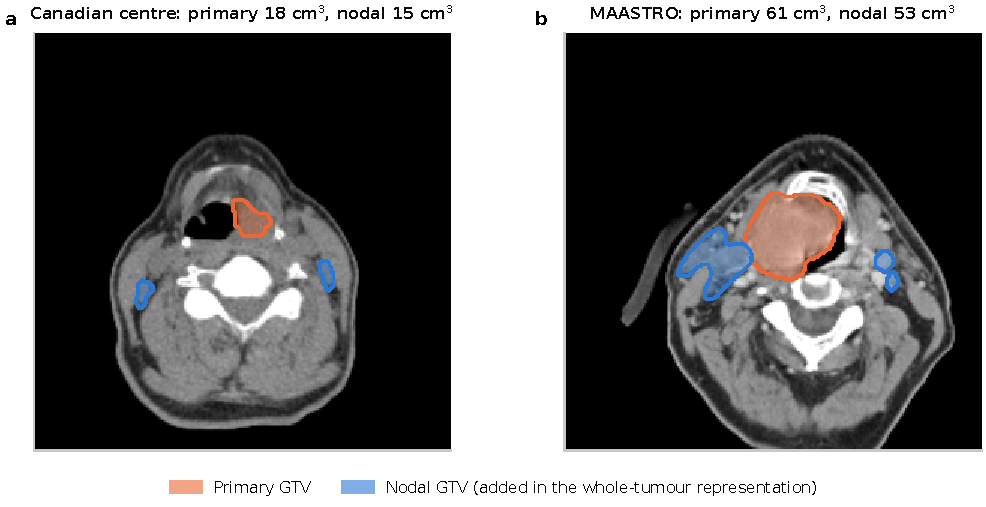
\includegraphics[width=0.92\textwidth]{Fig1.pdf}
\caption{Tumour definitions on pretreatment CT. Axial slices of one HN-PET-CT (\textbf{a}) and one HN1 (\textbf{b}) patient showing the primary GTV (orange), used alone in the primary-GTV representation, and the nodal GTVs (blue), added in the whole-tumour representation. Volumes refer to the complete structures. Images from the HN-PET-CT and HN1 collections~\cite{vallieres2017tcia,wee2019hn1}}\label{fig:ct}
\end{figure*}

\subsection{Whole-Tumour Graph Neural Network}\label{sec:gnn}
The proposed model combines the whole-tumour radiomic features of Section~\ref{sec:features} with a patient-similarity graph (Fig.~\ref{fig:arch}). The same networks trained on primary-GTV features are referred to as the primary-GTV variant.

\begin{figure*}[!tp]
\centering
\resizebox{\textwidth}{!}{% Whole-tumour GNN architecture: vector figure drawn in TikZ (no generated images).
% The CT slice is a crop of Fig. 1b (HN1 patient, primary GTV orange, nodal GTV blue): figures/ct_crop_hn1.png.
% Included in main.tex with % Whole-tumour GNN architecture: vector figure drawn in TikZ (no generated images).
% The CT slice is a crop of Fig. 1b (HN1 patient, primary GTV orange, nodal GTV blue): figures/ct_crop_hn1.png.
% Included in main.tex with % Whole-tumour GNN architecture: vector figure drawn in TikZ (no generated images).
% The CT slice is a crop of Fig. 1b (HN1 patient, primary GTV orange, nodal GTV blue): figures/ct_crop_hn1.png.
% Included in main.tex with \input{figures/Fig2}; needs tikz libraries
% arrows.meta, positioning, calc, fit, backgrounds, shapes.geometric and the macros of tables/numbers.tex.
\begin{tikzpicture}[
  font=\sffamily\fontsize{7}{8.4}\selectfont, >={Stealth[length=4pt]}, line width=0.6pt,
  hdr/.style={font=\sffamily\fontsize{8.5}{10}\selectfont\bfseries, anchor=west, text=#1!45!black},
  badge/.style={circle, fill=white, draw=#1!60!black, line width=0.8pt, text=#1!50!black,
                font=\sffamily\fontsize{8}{9}\selectfont\bfseries, inner sep=0pt, minimum size=13pt},
  blk/.style={draw=#1!60!black, fill=#1!20, rounded corners=2.5pt, align=center,
              minimum width=12mm, minimum height=12mm, inner sep=1pt, text width=11.5mm},
  note/.style={draw=#1!55!black, fill=white, rounded corners=3pt, align=left, inner sep=4pt},
  arr/.style={->, draw=black!70},
  stage/.style={-{Latex[length=7pt,width=9pt]}, line width=3.5pt, draw=black!35},
  tr0/.style={circle, draw=white, line width=0.5pt, fill=blue!65!cyan!80!black, minimum size=8pt, inner sep=0pt},
  tr1/.style={circle, draw=white, line width=0.5pt, fill=red!75!black, minimum size=8pt, inner sep=0pt},
  test/.style={star, star points=5, star point ratio=2.2, draw=black!80, fill=orange!85!yellow, minimum size=12pt, inner sep=0pt},
  plus/.style={circle, draw=black!70, fill=white, inner sep=0pt, minimum size=10pt, font=\sffamily\fontsize{8}{8}\selectfont\bfseries},
  lab/.style={font=\sffamily\fontsize{5.8}{6.6}\selectfont, text=black!70},
  cell/.style={draw=white, line width=0.6pt, minimum width=4.2mm, minimum height=4.6mm, inner sep=0pt},
  key/.style={minimum width=5pt, minimum height=5pt, inner sep=0pt, draw=orange!50!black},
]

%% ================================================================ stage backgrounds
\begin{scope}[on background layer]
  \fill[orange!7]  (0,0)    rectangle (4.6,9.4);   \fill[orange!28] (0,8.75) rectangle (4.6,9.4);
  \fill[blue!6]    (4.8,0)  rectangle (8.7,9.4);   \fill[blue!22]   (4.8,8.75) rectangle (8.7,9.4);
  \fill[teal!7]    (8.9,0)  rectangle (15.3,9.4);  \fill[teal!28]   (8.9,8.75) rectangle (15.3,9.4);
  \fill[violet!7]  (15.5,0) rectangle (18.0,9.4);  \fill[violet!22] (15.5,8.75) rectangle (18.0,9.4);
  \fill[yellow!12] (0,-2.75) rectangle (8.7,-0.2);
  \fill[black!6]   (8.9,-2.75) rectangle (18.0,-0.2);
\end{scope}
\node[badge=orange] at (0.35,9.075) {1}; \node[hdr=orange] at (0.6,9.075) {Whole-tumour radiomics};
\node[badge=blue]   at (5.15,9.075) {2}; \node[hdr=blue]   at (5.4,9.075) {Patient graph};
\node[badge=teal]   at (9.25,9.075) {3}; \node[hdr=teal]   at (9.5,9.075) {Graph neural network};
\node[badge=violet] at (15.85,9.075){4}; \node[hdr=violet] at (16.1,9.075) {Prediction};

%% ================================================================ 1  whole-tumour radiomics
\node[inner sep=0pt, draw=black!50] (ct) at (2.30,7.35) {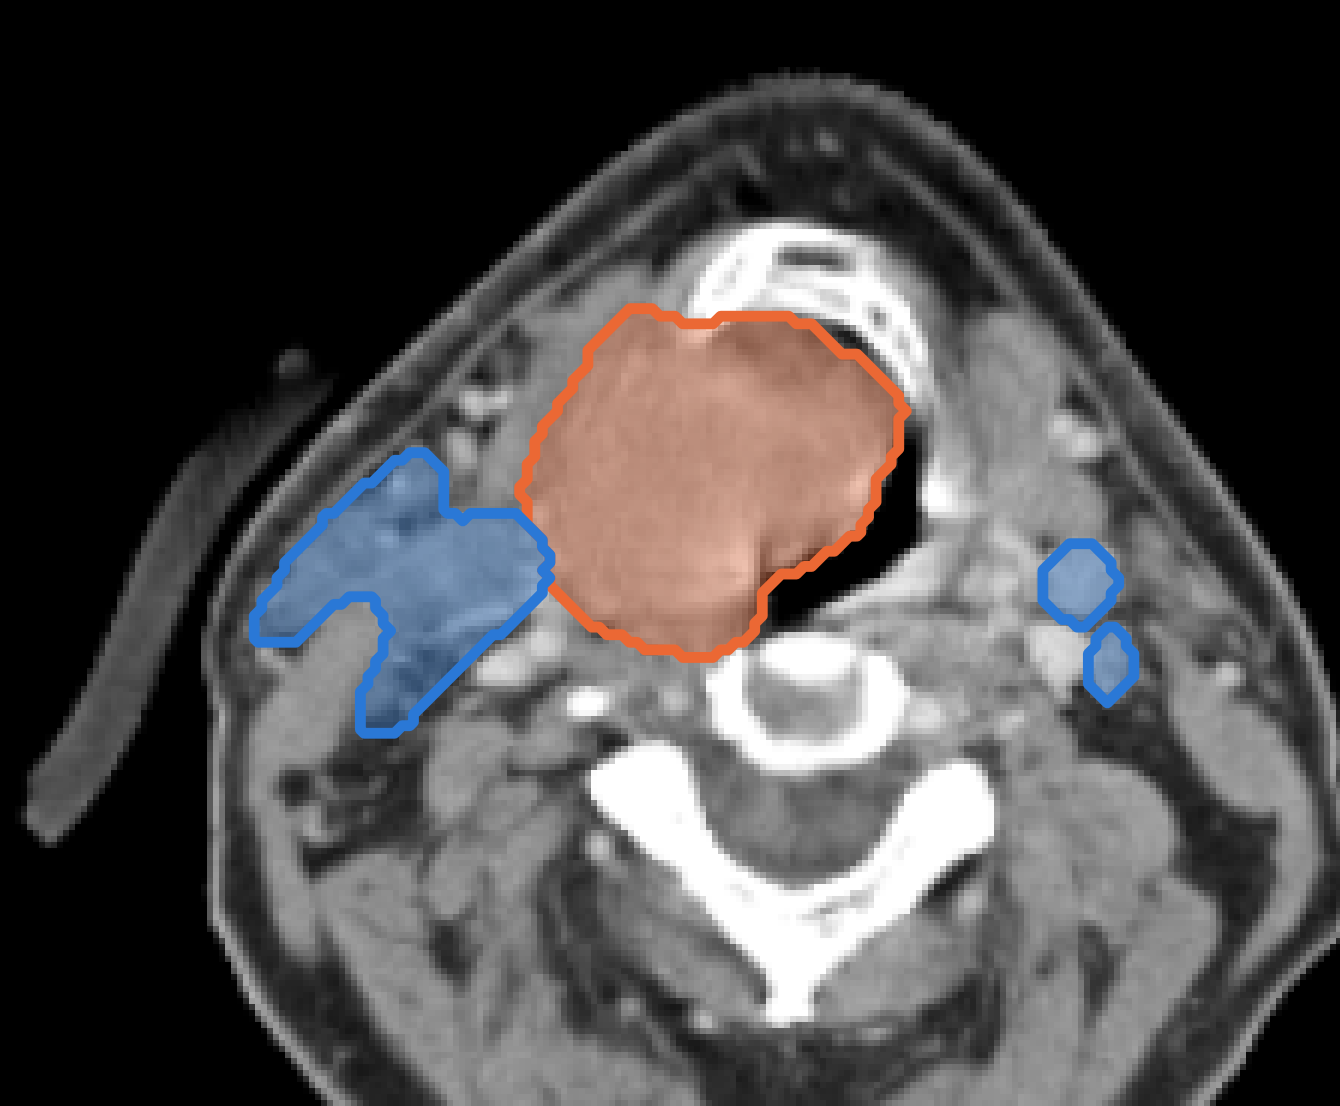
\includegraphics[width=3.1cm]{figures/ct_crop_hn1.png}};
\node[anchor=north, align=center] at (2.30,6.02) {%
  \tikz{\fill[orange!80!red, draw=orange!50!black] (0,0) rectangle (6pt,6pt);}\ primary GTV\enspace
  \tikz{\fill[blue!55!cyan, draw=blue!50!black] (0,0) rectangle (6pt,6pt);}\ nodal GTV\\[1pt]
  \textbf{whole tumour = primary $\cup$ nodal}};
\draw[arr] (2.30,5.28) -- (2.30,5.05);
% feature bar (widths proportional to 14 / 93 / 372 of 479 features)
\node[font=\sffamily\fontsize{7}{8}\selectfont\bfseries] at (2.30,4.85) {479 radiomic features (PyRadiomics)};
\fill[orange!75!black] (0.40,4.15) rectangle (0.52,4.60);
\fill[orange!55]       (0.52,4.15) rectangle (1.30,4.60);
\fill[orange!25]       (1.30,4.15) rectangle (4.20,4.60);
\draw[orange!50!black] (0.40,4.15) rectangle (4.20,4.60);
\node[lab, anchor=north, align=center] at (2.30,4.08) {%
  \tikz\node[key, fill=orange!75!black]{};\ shape 14\enspace
  \tikz\node[key, fill=orange!55]{};\ original 93\enspace
  \tikz\node[key, fill=orange!25]{};\ LoG-filtered 372};
\draw[arr] (2.30,3.68) -- (2.30,3.45);
% selection funnel
\filldraw[fill=orange!18, draw=orange!55!black, rounded corners=2pt] (0.30,3.42) -- (4.30,3.42) -- (3.50,2.42) -- (1.10,2.42) -- cycle;
\node[align=center, text width=3.4cm] at (2.30,2.95) {\textbf{Feature selection}\\mRMR, LASSO or filter\\on training data only};
\draw[arr] (2.30,2.42) -- (2.30,2.10);
% node feature vector
\foreach \i in {0,...,3} \node[cell, fill=orange!65] at (1.05+0.42*\i,1.82) {};
\foreach \i in {0,...,2} \node[cell, fill=green!55!black!70] at (2.85+0.42*\i,1.82) {};
\node[anchor=east, font=\sffamily\fontsize{8}{9}\selectfont\bfseries] at (0.80,1.82) {$\mathbf{x}_i$};
\node[lab, anchor=north, align=center] at (1.68,1.52) {2, 4 or 8\\radiomic};
\node[lab, anchor=north, align=center] at (3.27,1.52) {T, N, volume\\(optional)};
\node[anchor=south, align=center, text=orange!40!black] at (2.30,0.12) {\textbf{one feature vector per patient}};

%% ================================================================ 2  patient-similarity graph
\begin{scope}[shift={(5.15,4.15)}]
  \node[tr0] (p1) at (0.30, 3.40) {};
  \node[tr0] (p2) at (1.25, 3.85) {};
  \node[tr1] (p3) at (2.30, 3.55) {};
  \node[tr0] (p4) at (3.20, 3.95) {};
  \node[tr0] (p5) at (0.55, 2.35) {};
  \node[tr1] (p6) at (1.60, 2.75) {};
  \node[tr0] (p7) at (2.95, 2.70) {};
  \node[tr0] (p8) at (0.25, 1.20) {};
  \node[tr0] (p9) at (2.70, 1.45) {};
  \node[tr1] (p10) at (3.25, 0.70) {};
  \node[tr0] (p11) at (1.00, 0.35) {};
  \node[test] (t1) at (1.60, 1.10) {};
  \begin{scope}[on background layer]
    \foreach \a/\b in {p1/p2, p2/p3, p3/p4, p1/p5, p2/p6, p5/p6, p3/p6, p4/p7, p3/p7, p6/p7, p5/p8, p7/p9, p9/p10, p7/p10, p6/p9, p8/p11, p11/p9}
      \draw[black!28, line width=0.5pt] (\a) -- (\b);
    \foreach \a in {p5, p6, p8, p9}
      \draw[orange!85!black, line width=0.9pt, ->, >={Stealth[length=4pt]}, shorten >=2pt] (\a) -- (t1);
  \end{scope}
\end{scope}
\node[align=left, anchor=north west] at (5.00,4.00) {%
  \tikz\node[tr0]{};\ training patient, no event\\[1.5pt]
  \tikz\node[tr1]{};\ training patient, event\\[1.5pt]
  \tikz\node[test, minimum size=9pt]{};\ test patient (outcome unseen)};
\node[note=blue, text width=3.45cm, anchor=north] at (6.75,2.55) {%
  \textbf{Edges:} each patient receives links from its 5, 10 or 20 most similar \emph{training} patients (cosine similarity of $\mathbf{x}_i$).\\[2pt]
  \textbf{No leakage:} test patients receive links but never send them.};

%% ================================================================ 3  network
\begin{scope}[every node/.append style={}]
\node[blk=blue, text width=9.5mm, minimum width=10.5mm]   (in)  at (9.50,7.00)  {$\mathbf{x}_i$\\dropout\\0.2};
\node[blk=teal, text width=10mm, minimum width=11mm]      (mp1) at (10.85,7.00) {Message\\passing 1\\(32)};
\node[plus]                                               (s1)  at (11.78,7.00) {+};
\node[blk=teal, text width=10mm, minimum width=11mm]      (mp2) at (12.85,7.00) {Message\\passing 2\\(32)};
\node[plus]                                               (s2)  at (13.78,7.00) {+};
\node[blk=violet, text width=8.8mm, minimum width=9.4mm]      (out) at (14.75,7.00) {Linear\\+\\sigmoid};
\end{scope}
\draw[arr] (in) -- (mp1);
\draw[arr] (mp1) -- (s1);
\draw[arr] (s1) -- (mp2);
\draw[arr] (mp2) -- (s2);
\draw[arr] (s2) -- (out);
% linear skip: Linear(x) added to the output of message passing 1
\draw[arr, draw=black!55] (in.north) -- ++(0,0.42) -| node[pos=0.25, above, lab] {linear skip from input} (s1.north);
% residual: output of layer 1 (h1) added to the output of layer 2
\draw[arr, draw=teal!50!black] ($(s1.east)!0.5!(mp2.west)$) -- ++(0,0.72) -| node[pos=0.25, above, lab, text=teal!40!black] {residual} (s2.north);
\node[lab, align=center, text width=5.9cm] at (12.10,6.02) {Message passing: GCN, GraphSAGE or GAT (4 heads $\times$ 8).\\Each layer is followed by ELU and dropout 0.5.};
% inset: inside one message-passing layer
\node[note=teal, minimum width=6.1cm, minimum height=4.55cm, anchor=north west] (inset) at (9.05,5.55) {};
\node[anchor=north west, font=\sffamily\fontsize{7}{8}\selectfont\bfseries, text=teal!40!black] at (9.15,5.50) {Inside one message-passing layer};
\begin{scope}[shift={(10.25,3.35)}]
  \node[circle, fill=blue!65!cyan!80!black, draw=white, minimum size=17pt, inner sep=0pt, text=white, font=\sffamily\fontsize{7.5}{8}\selectfont\bfseries] (ci) at (0,0) {$i$};
  \node[tr0, minimum size=11pt, text=white, font=\sffamily\fontsize{5.5}{6}\selectfont] (j1) at (-0.85,0.90) {$j$};
  \node[tr1, minimum size=11pt, text=white, font=\sffamily\fontsize{5.5}{6}\selectfont] (j2) at (0.85,0.90) {$j$};
  \node[tr0, minimum size=11pt, text=white, font=\sffamily\fontsize{5.5}{6}\selectfont] (j3) at (-0.85,-0.90) {$j$};
  \node[tr0, minimum size=11pt, text=white, font=\sffamily\fontsize{5.5}{6}\selectfont] (j4) at (0.85,-0.90) {$j$};
  \foreach \j in {j1, j2, j3, j4}
    \draw[->, orange!85!black, line width=0.9pt, shorten >=1pt] (\j) -- (ci);
  \draw[->, black!60, line width=0.7pt] (ci.north east) .. controls +(0.5,0.35) and +(0.5,-0.35) .. (ci.south east);
  \node[lab] at (0.88,0) {self};
  \node[lab, align=center, anchor=north] at (0,-1.20) {neighbours $j$ = training\\patients linked to $i$};
\end{scope}
\node[anchor=north west, align=left, text width=3.55cm] at (11.45,4.95) {%
  Each patient's representation is updated from its own features and those of its neighbours:\\[5pt]
  $\mathbf{h}_i' = \mathbf{W}_0\mathbf{h}_i + \textstyle\sum_{j} w_{ij}\mathbf{W}\mathbf{h}_j$\\[5pt]
  $w_{ij}$: degree-normalised (GCN), mean (GraphSAGE) or learned attention (GAT).};
\node[align=center, text width=6.0cm, text=teal!35!black] at (12.10,0.50) {Training: full batch, 150 epochs, Adam (learning rate 0.005), class-weighted cross-entropy};

%% ================================================================ 4  prediction
\node[align=center, text width=2.3cm] at (16.75,8.15) {\textbf{Probability of event}\\for each patient};
\foreach \y/\e/\f/\c in {7.20/LR (2 y)/0.55/red, 6.35/DM (2 y)/0.30/orange, 5.50/OS (4 y)/0.70/violet}{
  \node[anchor=west] at (15.70,\y+0.28) {\e};
  \fill[black!12, rounded corners=1.5pt] (15.75,\y-0.12) rectangle (17.80,\y+0.08);
  \fill[\c!70!black, rounded corners=1.5pt] (15.75,\y-0.12) rectangle ({15.75+2.05*\f},\y+0.08);
}
\node[lab] at (16.78,4.98) {illustrative values};
\node[note=violet, text width=2.0cm, anchor=north, align=center] at (16.75,4.55) {%
  \textbf{Ten-seed ensemble}\\[2pt]
  \tikz{\foreach \k in {0,...,9} \fill[violet!55] (\k*0.17,0) rectangle +(0.13,0.22);}\\[1pt]
  probabilities averaged over seeds 0--9};
\node[note=violet, text width=2.0cm, anchor=north, align=center] at (16.75,2.45) {%
  \textbf{Evaluation}\\[1pt] AUC on the external HN1 cohort, compared with the published CNN};

%% ================================================================ stage arrows
\draw[stage] (4.35,6.70) -- (5.10,6.70);
\draw[stage] (8.45,7.00) -- (in.west);
\draw[stage] (out.east) -- (16.05,7.00);

%% ================================================================ validation design strip
\node[anchor=west, font=\sffamily\fontsize{7.5}{9}\selectfont\bfseries, text=yellow!25!black] at (0.20,-0.48) {Validation design};
\node[note=blue, text width=3.45cm, anchor=north west, fill=blue!8] (dev) at (0.20,-0.75) {%
  \textbf{Development:} HN-PET-CT, \nPatCan{} patients, four Canadian centres. 5-fold CV or cohort split; model chosen on validation AUC.};
\node[note=orange, text width=3.45cm, anchor=north west, fill=orange!10] (tst) at (4.75,-0.75) {%
  \textbf{External test:} HN1, \nPatMAA{} patients, MAASTRO Clinic. Never used for training or model selection.};
\draw[stage, line width=2.5pt] (dev.east) -- (tst.west);

%% ================================================================ no-edge control strip
\node[anchor=west, font=\sffamily\fontsize{7.5}{9}\selectfont\bfseries, text=black!65] at (9.05,-0.48) {No-edge control (MLP)};
\begin{scope}[every node/.append style={minimum height=8mm, text width=9mm, minimum width=10mm}]
  \node[blk=blue]   (cin) at (9.50,-1.60) {$\mathbf{x}_i$};
  \node[blk=gray]   (l1)  at (10.85,-1.60) {Linear 1\\(32)};
  \node[blk=gray]   (l2)  at (12.85,-1.60) {Linear 2\\(32)};
\end{scope}
\node[plus] (cs1) at (11.78,-1.60) {+};
\node[plus] (cs2) at (13.78,-1.60) {+};
\node[blk=violet, minimum height=8mm, text width=8.8mm, minimum width=9.4mm] (co) at (14.75,-1.60) {Linear +\\sigmoid};
\draw[arr] (cin) -- (l1); \draw[arr] (l1) -- (cs1); \draw[arr] (cs1) -- (l2); \draw[arr] (l2) -- (cs2); \draw[arr] (cs2) -- (co);
\draw[arr, draw=black!55] (cin.north) -- ++(0,0.25) -| (cs1.north);
\draw[arr, draw=teal!50!black] ($(cs1.east)!0.5!(l2.west)$) -- ++(0,0.65) -| (cs2.north);
\node[anchor=west, align=left, text width=2.45cm] at (15.30,-1.50) {Identical network with linear layers in place of message passing, so the graph is ignored. Comparing the two shows what the graph adds.};
\end{tikzpicture}
; needs tikz libraries
% arrows.meta, positioning, calc, fit, backgrounds, shapes.geometric and the macros of tables/numbers.tex.
\begin{tikzpicture}[
  font=\sffamily\fontsize{7}{8.4}\selectfont, >={Stealth[length=4pt]}, line width=0.6pt,
  hdr/.style={font=\sffamily\fontsize{8.5}{10}\selectfont\bfseries, anchor=west, text=#1!45!black},
  badge/.style={circle, fill=white, draw=#1!60!black, line width=0.8pt, text=#1!50!black,
                font=\sffamily\fontsize{8}{9}\selectfont\bfseries, inner sep=0pt, minimum size=13pt},
  blk/.style={draw=#1!60!black, fill=#1!20, rounded corners=2.5pt, align=center,
              minimum width=12mm, minimum height=12mm, inner sep=1pt, text width=11.5mm},
  note/.style={draw=#1!55!black, fill=white, rounded corners=3pt, align=left, inner sep=4pt},
  arr/.style={->, draw=black!70},
  stage/.style={-{Latex[length=7pt,width=9pt]}, line width=3.5pt, draw=black!35},
  tr0/.style={circle, draw=white, line width=0.5pt, fill=blue!65!cyan!80!black, minimum size=8pt, inner sep=0pt},
  tr1/.style={circle, draw=white, line width=0.5pt, fill=red!75!black, minimum size=8pt, inner sep=0pt},
  test/.style={star, star points=5, star point ratio=2.2, draw=black!80, fill=orange!85!yellow, minimum size=12pt, inner sep=0pt},
  plus/.style={circle, draw=black!70, fill=white, inner sep=0pt, minimum size=10pt, font=\sffamily\fontsize{8}{8}\selectfont\bfseries},
  lab/.style={font=\sffamily\fontsize{5.8}{6.6}\selectfont, text=black!70},
  cell/.style={draw=white, line width=0.6pt, minimum width=4.2mm, minimum height=4.6mm, inner sep=0pt},
  key/.style={minimum width=5pt, minimum height=5pt, inner sep=0pt, draw=orange!50!black},
]

%% ================================================================ stage backgrounds
\begin{scope}[on background layer]
  \fill[orange!7]  (0,0)    rectangle (4.6,9.4);   \fill[orange!28] (0,8.75) rectangle (4.6,9.4);
  \fill[blue!6]    (4.8,0)  rectangle (8.7,9.4);   \fill[blue!22]   (4.8,8.75) rectangle (8.7,9.4);
  \fill[teal!7]    (8.9,0)  rectangle (15.3,9.4);  \fill[teal!28]   (8.9,8.75) rectangle (15.3,9.4);
  \fill[violet!7]  (15.5,0) rectangle (18.0,9.4);  \fill[violet!22] (15.5,8.75) rectangle (18.0,9.4);
  \fill[yellow!12] (0,-2.75) rectangle (8.7,-0.2);
  \fill[black!6]   (8.9,-2.75) rectangle (18.0,-0.2);
\end{scope}
\node[badge=orange] at (0.35,9.075) {1}; \node[hdr=orange] at (0.6,9.075) {Whole-tumour radiomics};
\node[badge=blue]   at (5.15,9.075) {2}; \node[hdr=blue]   at (5.4,9.075) {Patient graph};
\node[badge=teal]   at (9.25,9.075) {3}; \node[hdr=teal]   at (9.5,9.075) {Graph neural network};
\node[badge=violet] at (15.85,9.075){4}; \node[hdr=violet] at (16.1,9.075) {Prediction};

%% ================================================================ 1  whole-tumour radiomics
\node[inner sep=0pt, draw=black!50] (ct) at (2.30,7.35) {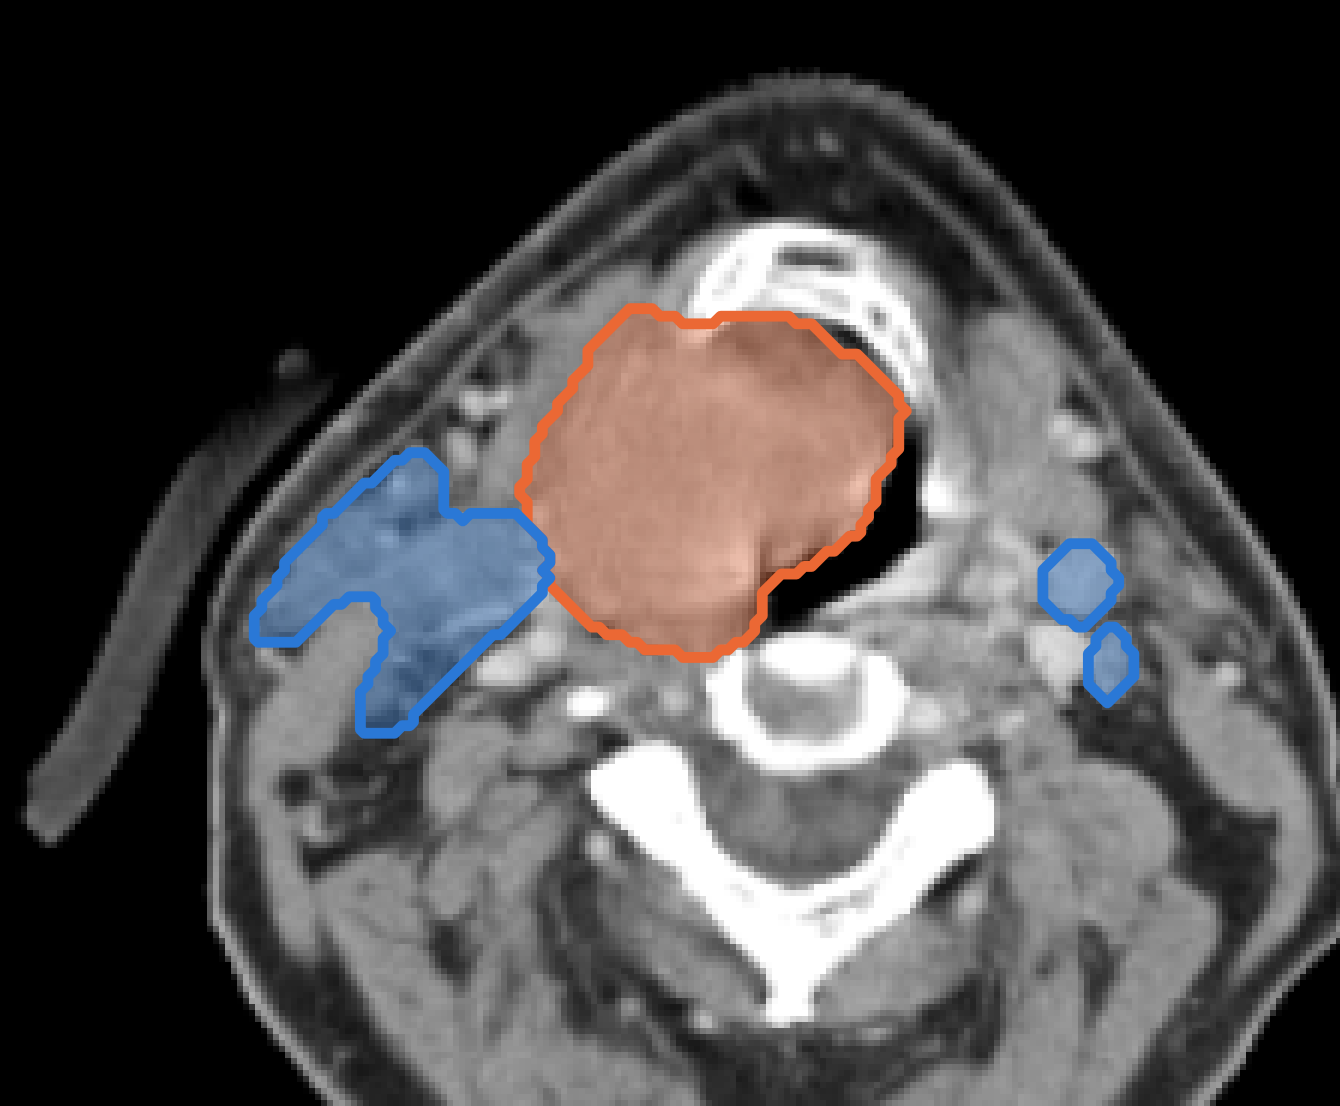
\includegraphics[width=3.1cm]{figures/ct_crop_hn1.png}};
\node[anchor=north, align=center] at (2.30,6.02) {%
  \tikz{\fill[orange!80!red, draw=orange!50!black] (0,0) rectangle (6pt,6pt);}\ primary GTV\enspace
  \tikz{\fill[blue!55!cyan, draw=blue!50!black] (0,0) rectangle (6pt,6pt);}\ nodal GTV\\[1pt]
  \textbf{whole tumour = primary $\cup$ nodal}};
\draw[arr] (2.30,5.28) -- (2.30,5.05);
% feature bar (widths proportional to 14 / 93 / 372 of 479 features)
\node[font=\sffamily\fontsize{7}{8}\selectfont\bfseries] at (2.30,4.85) {479 radiomic features (PyRadiomics)};
\fill[orange!75!black] (0.40,4.15) rectangle (0.52,4.60);
\fill[orange!55]       (0.52,4.15) rectangle (1.30,4.60);
\fill[orange!25]       (1.30,4.15) rectangle (4.20,4.60);
\draw[orange!50!black] (0.40,4.15) rectangle (4.20,4.60);
\node[lab, anchor=north, align=center] at (2.30,4.08) {%
  \tikz\node[key, fill=orange!75!black]{};\ shape 14\enspace
  \tikz\node[key, fill=orange!55]{};\ original 93\enspace
  \tikz\node[key, fill=orange!25]{};\ LoG-filtered 372};
\draw[arr] (2.30,3.68) -- (2.30,3.45);
% selection funnel
\filldraw[fill=orange!18, draw=orange!55!black, rounded corners=2pt] (0.30,3.42) -- (4.30,3.42) -- (3.50,2.42) -- (1.10,2.42) -- cycle;
\node[align=center, text width=3.4cm] at (2.30,2.95) {\textbf{Feature selection}\\mRMR, LASSO or filter\\on training data only};
\draw[arr] (2.30,2.42) -- (2.30,2.10);
% node feature vector
\foreach \i in {0,...,3} \node[cell, fill=orange!65] at (1.05+0.42*\i,1.82) {};
\foreach \i in {0,...,2} \node[cell, fill=green!55!black!70] at (2.85+0.42*\i,1.82) {};
\node[anchor=east, font=\sffamily\fontsize{8}{9}\selectfont\bfseries] at (0.80,1.82) {$\mathbf{x}_i$};
\node[lab, anchor=north, align=center] at (1.68,1.52) {2, 4 or 8\\radiomic};
\node[lab, anchor=north, align=center] at (3.27,1.52) {T, N, volume\\(optional)};
\node[anchor=south, align=center, text=orange!40!black] at (2.30,0.12) {\textbf{one feature vector per patient}};

%% ================================================================ 2  patient-similarity graph
\begin{scope}[shift={(5.15,4.15)}]
  \node[tr0] (p1) at (0.30, 3.40) {};
  \node[tr0] (p2) at (1.25, 3.85) {};
  \node[tr1] (p3) at (2.30, 3.55) {};
  \node[tr0] (p4) at (3.20, 3.95) {};
  \node[tr0] (p5) at (0.55, 2.35) {};
  \node[tr1] (p6) at (1.60, 2.75) {};
  \node[tr0] (p7) at (2.95, 2.70) {};
  \node[tr0] (p8) at (0.25, 1.20) {};
  \node[tr0] (p9) at (2.70, 1.45) {};
  \node[tr1] (p10) at (3.25, 0.70) {};
  \node[tr0] (p11) at (1.00, 0.35) {};
  \node[test] (t1) at (1.60, 1.10) {};
  \begin{scope}[on background layer]
    \foreach \a/\b in {p1/p2, p2/p3, p3/p4, p1/p5, p2/p6, p5/p6, p3/p6, p4/p7, p3/p7, p6/p7, p5/p8, p7/p9, p9/p10, p7/p10, p6/p9, p8/p11, p11/p9}
      \draw[black!28, line width=0.5pt] (\a) -- (\b);
    \foreach \a in {p5, p6, p8, p9}
      \draw[orange!85!black, line width=0.9pt, ->, >={Stealth[length=4pt]}, shorten >=2pt] (\a) -- (t1);
  \end{scope}
\end{scope}
\node[align=left, anchor=north west] at (5.00,4.00) {%
  \tikz\node[tr0]{};\ training patient, no event\\[1.5pt]
  \tikz\node[tr1]{};\ training patient, event\\[1.5pt]
  \tikz\node[test, minimum size=9pt]{};\ test patient (outcome unseen)};
\node[note=blue, text width=3.45cm, anchor=north] at (6.75,2.55) {%
  \textbf{Edges:} each patient receives links from its 5, 10 or 20 most similar \emph{training} patients (cosine similarity of $\mathbf{x}_i$).\\[2pt]
  \textbf{No leakage:} test patients receive links but never send them.};

%% ================================================================ 3  network
\begin{scope}[every node/.append style={}]
\node[blk=blue, text width=9.5mm, minimum width=10.5mm]   (in)  at (9.50,7.00)  {$\mathbf{x}_i$\\dropout\\0.2};
\node[blk=teal, text width=10mm, minimum width=11mm]      (mp1) at (10.85,7.00) {Message\\passing 1\\(32)};
\node[plus]                                               (s1)  at (11.78,7.00) {+};
\node[blk=teal, text width=10mm, minimum width=11mm]      (mp2) at (12.85,7.00) {Message\\passing 2\\(32)};
\node[plus]                                               (s2)  at (13.78,7.00) {+};
\node[blk=violet, text width=8.8mm, minimum width=9.4mm]      (out) at (14.75,7.00) {Linear\\+\\sigmoid};
\end{scope}
\draw[arr] (in) -- (mp1);
\draw[arr] (mp1) -- (s1);
\draw[arr] (s1) -- (mp2);
\draw[arr] (mp2) -- (s2);
\draw[arr] (s2) -- (out);
% linear skip: Linear(x) added to the output of message passing 1
\draw[arr, draw=black!55] (in.north) -- ++(0,0.42) -| node[pos=0.25, above, lab] {linear skip from input} (s1.north);
% residual: output of layer 1 (h1) added to the output of layer 2
\draw[arr, draw=teal!50!black] ($(s1.east)!0.5!(mp2.west)$) -- ++(0,0.72) -| node[pos=0.25, above, lab, text=teal!40!black] {residual} (s2.north);
\node[lab, align=center, text width=5.9cm] at (12.10,6.02) {Message passing: GCN, GraphSAGE or GAT (4 heads $\times$ 8).\\Each layer is followed by ELU and dropout 0.5.};
% inset: inside one message-passing layer
\node[note=teal, minimum width=6.1cm, minimum height=4.55cm, anchor=north west] (inset) at (9.05,5.55) {};
\node[anchor=north west, font=\sffamily\fontsize{7}{8}\selectfont\bfseries, text=teal!40!black] at (9.15,5.50) {Inside one message-passing layer};
\begin{scope}[shift={(10.25,3.35)}]
  \node[circle, fill=blue!65!cyan!80!black, draw=white, minimum size=17pt, inner sep=0pt, text=white, font=\sffamily\fontsize{7.5}{8}\selectfont\bfseries] (ci) at (0,0) {$i$};
  \node[tr0, minimum size=11pt, text=white, font=\sffamily\fontsize{5.5}{6}\selectfont] (j1) at (-0.85,0.90) {$j$};
  \node[tr1, minimum size=11pt, text=white, font=\sffamily\fontsize{5.5}{6}\selectfont] (j2) at (0.85,0.90) {$j$};
  \node[tr0, minimum size=11pt, text=white, font=\sffamily\fontsize{5.5}{6}\selectfont] (j3) at (-0.85,-0.90) {$j$};
  \node[tr0, minimum size=11pt, text=white, font=\sffamily\fontsize{5.5}{6}\selectfont] (j4) at (0.85,-0.90) {$j$};
  \foreach \j in {j1, j2, j3, j4}
    \draw[->, orange!85!black, line width=0.9pt, shorten >=1pt] (\j) -- (ci);
  \draw[->, black!60, line width=0.7pt] (ci.north east) .. controls +(0.5,0.35) and +(0.5,-0.35) .. (ci.south east);
  \node[lab] at (0.88,0) {self};
  \node[lab, align=center, anchor=north] at (0,-1.20) {neighbours $j$ = training\\patients linked to $i$};
\end{scope}
\node[anchor=north west, align=left, text width=3.55cm] at (11.45,4.95) {%
  Each patient's representation is updated from its own features and those of its neighbours:\\[5pt]
  $\mathbf{h}_i' = \mathbf{W}_0\mathbf{h}_i + \textstyle\sum_{j} w_{ij}\mathbf{W}\mathbf{h}_j$\\[5pt]
  $w_{ij}$: degree-normalised (GCN), mean (GraphSAGE) or learned attention (GAT).};
\node[align=center, text width=6.0cm, text=teal!35!black] at (12.10,0.50) {Training: full batch, 150 epochs, Adam (learning rate 0.005), class-weighted cross-entropy};

%% ================================================================ 4  prediction
\node[align=center, text width=2.3cm] at (16.75,8.15) {\textbf{Probability of event}\\for each patient};
\foreach \y/\e/\f/\c in {7.20/LR (2 y)/0.55/red, 6.35/DM (2 y)/0.30/orange, 5.50/OS (4 y)/0.70/violet}{
  \node[anchor=west] at (15.70,\y+0.28) {\e};
  \fill[black!12, rounded corners=1.5pt] (15.75,\y-0.12) rectangle (17.80,\y+0.08);
  \fill[\c!70!black, rounded corners=1.5pt] (15.75,\y-0.12) rectangle ({15.75+2.05*\f},\y+0.08);
}
\node[lab] at (16.78,4.98) {illustrative values};
\node[note=violet, text width=2.0cm, anchor=north, align=center] at (16.75,4.55) {%
  \textbf{Ten-seed ensemble}\\[2pt]
  \tikz{\foreach \k in {0,...,9} \fill[violet!55] (\k*0.17,0) rectangle +(0.13,0.22);}\\[1pt]
  probabilities averaged over seeds 0--9};
\node[note=violet, text width=2.0cm, anchor=north, align=center] at (16.75,2.45) {%
  \textbf{Evaluation}\\[1pt] AUC on the external HN1 cohort, compared with the published CNN};

%% ================================================================ stage arrows
\draw[stage] (4.35,6.70) -- (5.10,6.70);
\draw[stage] (8.45,7.00) -- (in.west);
\draw[stage] (out.east) -- (16.05,7.00);

%% ================================================================ validation design strip
\node[anchor=west, font=\sffamily\fontsize{7.5}{9}\selectfont\bfseries, text=yellow!25!black] at (0.20,-0.48) {Validation design};
\node[note=blue, text width=3.45cm, anchor=north west, fill=blue!8] (dev) at (0.20,-0.75) {%
  \textbf{Development:} HN-PET-CT, \nPatCan{} patients, four Canadian centres. 5-fold CV or cohort split; model chosen on validation AUC.};
\node[note=orange, text width=3.45cm, anchor=north west, fill=orange!10] (tst) at (4.75,-0.75) {%
  \textbf{External test:} HN1, \nPatMAA{} patients, MAASTRO Clinic. Never used for training or model selection.};
\draw[stage, line width=2.5pt] (dev.east) -- (tst.west);

%% ================================================================ no-edge control strip
\node[anchor=west, font=\sffamily\fontsize{7.5}{9}\selectfont\bfseries, text=black!65] at (9.05,-0.48) {No-edge control (MLP)};
\begin{scope}[every node/.append style={minimum height=8mm, text width=9mm, minimum width=10mm}]
  \node[blk=blue]   (cin) at (9.50,-1.60) {$\mathbf{x}_i$};
  \node[blk=gray]   (l1)  at (10.85,-1.60) {Linear 1\\(32)};
  \node[blk=gray]   (l2)  at (12.85,-1.60) {Linear 2\\(32)};
\end{scope}
\node[plus] (cs1) at (11.78,-1.60) {+};
\node[plus] (cs2) at (13.78,-1.60) {+};
\node[blk=violet, minimum height=8mm, text width=8.8mm, minimum width=9.4mm] (co) at (14.75,-1.60) {Linear +\\sigmoid};
\draw[arr] (cin) -- (l1); \draw[arr] (l1) -- (cs1); \draw[arr] (cs1) -- (l2); \draw[arr] (l2) -- (cs2); \draw[arr] (cs2) -- (co);
\draw[arr, draw=black!55] (cin.north) -- ++(0,0.25) -| (cs1.north);
\draw[arr, draw=teal!50!black] ($(cs1.east)!0.5!(l2.west)$) -- ++(0,0.65) -| (cs2.north);
\node[anchor=west, align=left, text width=2.45cm] at (15.30,-1.50) {Identical network with linear layers in place of message passing, so the graph is ignored. Comparing the two shows what the graph adds.};
\end{tikzpicture}
; needs tikz libraries
% arrows.meta, positioning, calc, fit, backgrounds, shapes.geometric and the macros of tables/numbers.tex.
\begin{tikzpicture}[
  font=\sffamily\fontsize{7}{8.4}\selectfont, >={Stealth[length=4pt]}, line width=0.6pt,
  hdr/.style={font=\sffamily\fontsize{8.5}{10}\selectfont\bfseries, anchor=west, text=#1!45!black},
  badge/.style={circle, fill=white, draw=#1!60!black, line width=0.8pt, text=#1!50!black,
                font=\sffamily\fontsize{8}{9}\selectfont\bfseries, inner sep=0pt, minimum size=13pt},
  blk/.style={draw=#1!60!black, fill=#1!20, rounded corners=2.5pt, align=center,
              minimum width=12mm, minimum height=12mm, inner sep=1pt, text width=11.5mm},
  note/.style={draw=#1!55!black, fill=white, rounded corners=3pt, align=left, inner sep=4pt},
  arr/.style={->, draw=black!70},
  stage/.style={-{Latex[length=7pt,width=9pt]}, line width=3.5pt, draw=black!35},
  tr0/.style={circle, draw=white, line width=0.5pt, fill=blue!65!cyan!80!black, minimum size=8pt, inner sep=0pt},
  tr1/.style={circle, draw=white, line width=0.5pt, fill=red!75!black, minimum size=8pt, inner sep=0pt},
  test/.style={star, star points=5, star point ratio=2.2, draw=black!80, fill=orange!85!yellow, minimum size=12pt, inner sep=0pt},
  plus/.style={circle, draw=black!70, fill=white, inner sep=0pt, minimum size=10pt, font=\sffamily\fontsize{8}{8}\selectfont\bfseries},
  lab/.style={font=\sffamily\fontsize{5.8}{6.6}\selectfont, text=black!70},
  cell/.style={draw=white, line width=0.6pt, minimum width=4.2mm, minimum height=4.6mm, inner sep=0pt},
  key/.style={minimum width=5pt, minimum height=5pt, inner sep=0pt, draw=orange!50!black},
]

%% ================================================================ stage backgrounds
\begin{scope}[on background layer]
  \fill[orange!7]  (0,0)    rectangle (4.6,9.4);   \fill[orange!28] (0,8.75) rectangle (4.6,9.4);
  \fill[blue!6]    (4.8,0)  rectangle (8.7,9.4);   \fill[blue!22]   (4.8,8.75) rectangle (8.7,9.4);
  \fill[teal!7]    (8.9,0)  rectangle (15.3,9.4);  \fill[teal!28]   (8.9,8.75) rectangle (15.3,9.4);
  \fill[violet!7]  (15.5,0) rectangle (18.0,9.4);  \fill[violet!22] (15.5,8.75) rectangle (18.0,9.4);
  \fill[yellow!12] (0,-2.75) rectangle (8.7,-0.2);
  \fill[black!6]   (8.9,-2.75) rectangle (18.0,-0.2);
\end{scope}
\node[badge=orange] at (0.35,9.075) {1}; \node[hdr=orange] at (0.6,9.075) {Whole-tumour radiomics};
\node[badge=blue]   at (5.15,9.075) {2}; \node[hdr=blue]   at (5.4,9.075) {Patient graph};
\node[badge=teal]   at (9.25,9.075) {3}; \node[hdr=teal]   at (9.5,9.075) {Graph neural network};
\node[badge=violet] at (15.85,9.075){4}; \node[hdr=violet] at (16.1,9.075) {Prediction};

%% ================================================================ 1  whole-tumour radiomics
\node[inner sep=0pt, draw=black!50] (ct) at (2.30,7.35) {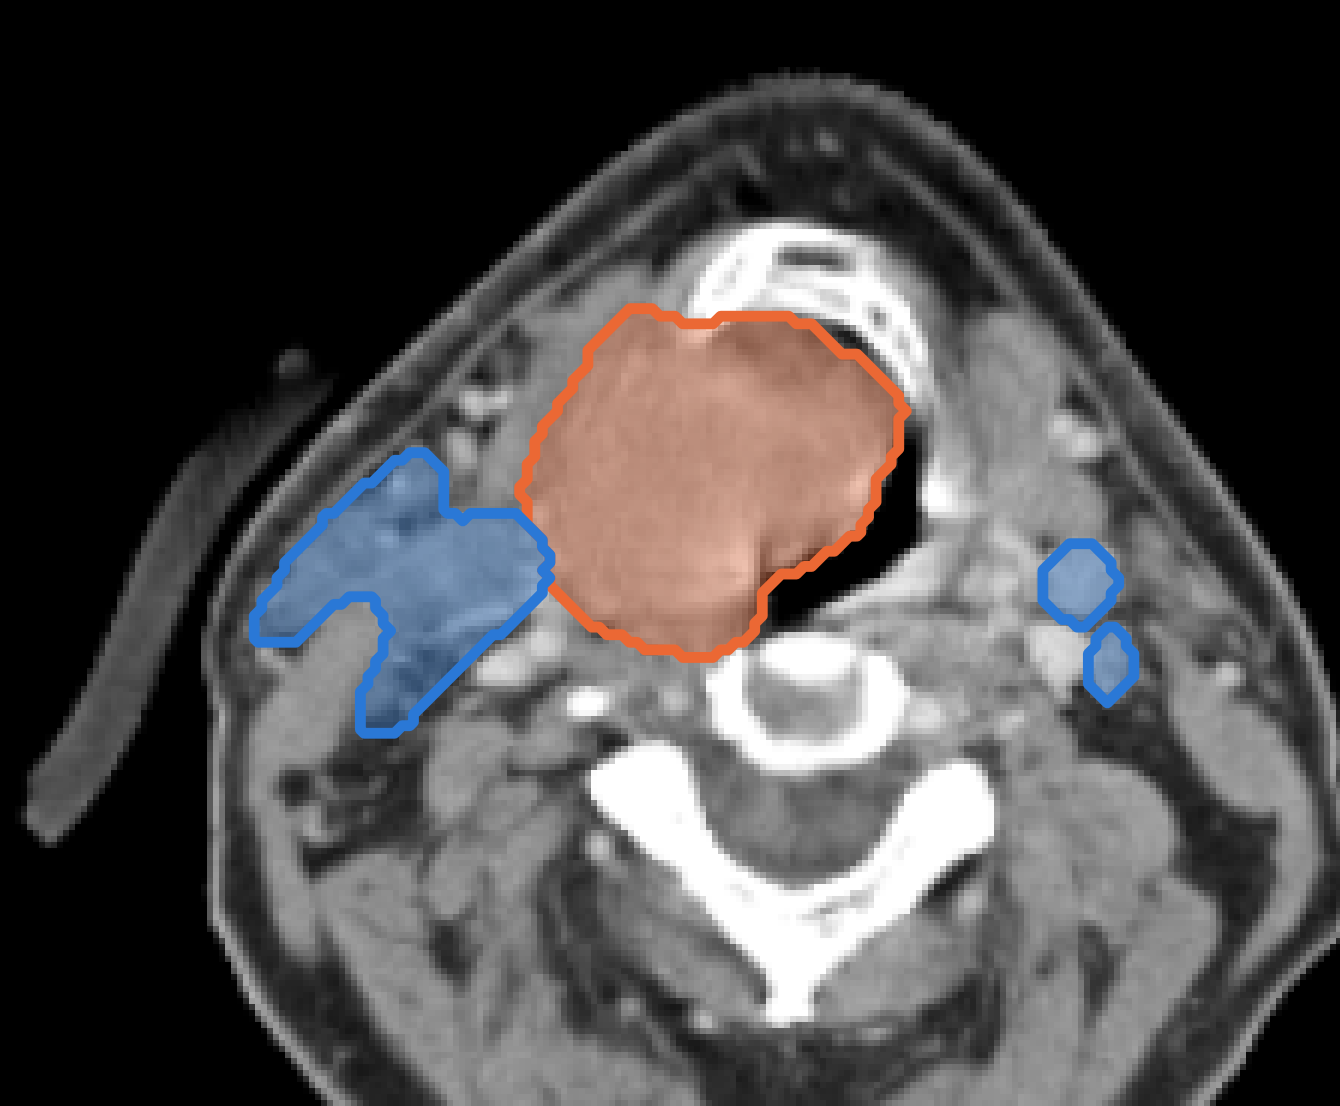
\includegraphics[width=3.1cm]{figures/ct_crop_hn1.png}};
\node[anchor=north, align=center] at (2.30,6.02) {%
  \tikz{\fill[orange!80!red, draw=orange!50!black] (0,0) rectangle (6pt,6pt);}\ primary GTV\enspace
  \tikz{\fill[blue!55!cyan, draw=blue!50!black] (0,0) rectangle (6pt,6pt);}\ nodal GTV\\[1pt]
  \textbf{whole tumour = primary $\cup$ nodal}};
\draw[arr] (2.30,5.28) -- (2.30,5.05);
% feature bar (widths proportional to 14 / 93 / 372 of 479 features)
\node[font=\sffamily\fontsize{7}{8}\selectfont\bfseries] at (2.30,4.85) {479 radiomic features (PyRadiomics)};
\fill[orange!75!black] (0.40,4.15) rectangle (0.52,4.60);
\fill[orange!55]       (0.52,4.15) rectangle (1.30,4.60);
\fill[orange!25]       (1.30,4.15) rectangle (4.20,4.60);
\draw[orange!50!black] (0.40,4.15) rectangle (4.20,4.60);
\node[lab, anchor=north, align=center] at (2.30,4.08) {%
  \tikz\node[key, fill=orange!75!black]{};\ shape 14\enspace
  \tikz\node[key, fill=orange!55]{};\ original 93\enspace
  \tikz\node[key, fill=orange!25]{};\ LoG-filtered 372};
\draw[arr] (2.30,3.68) -- (2.30,3.45);
% selection funnel
\filldraw[fill=orange!18, draw=orange!55!black, rounded corners=2pt] (0.30,3.42) -- (4.30,3.42) -- (3.50,2.42) -- (1.10,2.42) -- cycle;
\node[align=center, text width=3.4cm] at (2.30,2.95) {\textbf{Feature selection}\\mRMR, LASSO or filter\\on training data only};
\draw[arr] (2.30,2.42) -- (2.30,2.10);
% node feature vector
\foreach \i in {0,...,3} \node[cell, fill=orange!65] at (1.05+0.42*\i,1.82) {};
\foreach \i in {0,...,2} \node[cell, fill=green!55!black!70] at (2.85+0.42*\i,1.82) {};
\node[anchor=east, font=\sffamily\fontsize{8}{9}\selectfont\bfseries] at (0.80,1.82) {$\mathbf{x}_i$};
\node[lab, anchor=north, align=center] at (1.68,1.52) {2, 4 or 8\\radiomic};
\node[lab, anchor=north, align=center] at (3.27,1.52) {T, N, volume\\(optional)};
\node[anchor=south, align=center, text=orange!40!black] at (2.30,0.12) {\textbf{one feature vector per patient}};

%% ================================================================ 2  patient-similarity graph
\begin{scope}[shift={(5.15,4.15)}]
  \node[tr0] (p1) at (0.30, 3.40) {};
  \node[tr0] (p2) at (1.25, 3.85) {};
  \node[tr1] (p3) at (2.30, 3.55) {};
  \node[tr0] (p4) at (3.20, 3.95) {};
  \node[tr0] (p5) at (0.55, 2.35) {};
  \node[tr1] (p6) at (1.60, 2.75) {};
  \node[tr0] (p7) at (2.95, 2.70) {};
  \node[tr0] (p8) at (0.25, 1.20) {};
  \node[tr0] (p9) at (2.70, 1.45) {};
  \node[tr1] (p10) at (3.25, 0.70) {};
  \node[tr0] (p11) at (1.00, 0.35) {};
  \node[test] (t1) at (1.60, 1.10) {};
  \begin{scope}[on background layer]
    \foreach \a/\b in {p1/p2, p2/p3, p3/p4, p1/p5, p2/p6, p5/p6, p3/p6, p4/p7, p3/p7, p6/p7, p5/p8, p7/p9, p9/p10, p7/p10, p6/p9, p8/p11, p11/p9}
      \draw[black!28, line width=0.5pt] (\a) -- (\b);
    \foreach \a in {p5, p6, p8, p9}
      \draw[orange!85!black, line width=0.9pt, ->, >={Stealth[length=4pt]}, shorten >=2pt] (\a) -- (t1);
  \end{scope}
\end{scope}
\node[align=left, anchor=north west] at (5.00,4.00) {%
  \tikz\node[tr0]{};\ training patient, no event\\[1.5pt]
  \tikz\node[tr1]{};\ training patient, event\\[1.5pt]
  \tikz\node[test, minimum size=9pt]{};\ test patient (outcome unseen)};
\node[note=blue, text width=3.45cm, anchor=north] at (6.75,2.55) {%
  \textbf{Edges:} each patient receives links from its 5, 10 or 20 most similar \emph{training} patients (cosine similarity of $\mathbf{x}_i$).\\[2pt]
  \textbf{No leakage:} test patients receive links but never send them.};

%% ================================================================ 3  network
\begin{scope}[every node/.append style={}]
\node[blk=blue, text width=9.5mm, minimum width=10.5mm]   (in)  at (9.50,7.00)  {$\mathbf{x}_i$\\dropout\\0.2};
\node[blk=teal, text width=10mm, minimum width=11mm]      (mp1) at (10.85,7.00) {Message\\passing 1\\(32)};
\node[plus]                                               (s1)  at (11.78,7.00) {+};
\node[blk=teal, text width=10mm, minimum width=11mm]      (mp2) at (12.85,7.00) {Message\\passing 2\\(32)};
\node[plus]                                               (s2)  at (13.78,7.00) {+};
\node[blk=violet, text width=8.8mm, minimum width=9.4mm]      (out) at (14.75,7.00) {Linear\\+\\sigmoid};
\end{scope}
\draw[arr] (in) -- (mp1);
\draw[arr] (mp1) -- (s1);
\draw[arr] (s1) -- (mp2);
\draw[arr] (mp2) -- (s2);
\draw[arr] (s2) -- (out);
% linear skip: Linear(x) added to the output of message passing 1
\draw[arr, draw=black!55] (in.north) -- ++(0,0.42) -| node[pos=0.25, above, lab] {linear skip from input} (s1.north);
% residual: output of layer 1 (h1) added to the output of layer 2
\draw[arr, draw=teal!50!black] ($(s1.east)!0.5!(mp2.west)$) -- ++(0,0.72) -| node[pos=0.25, above, lab, text=teal!40!black] {residual} (s2.north);
\node[lab, align=center, text width=5.9cm] at (12.10,6.02) {Message passing: GCN, GraphSAGE or GAT (4 heads $\times$ 8).\\Each layer is followed by ELU and dropout 0.5.};
% inset: inside one message-passing layer
\node[note=teal, minimum width=6.1cm, minimum height=4.55cm, anchor=north west] (inset) at (9.05,5.55) {};
\node[anchor=north west, font=\sffamily\fontsize{7}{8}\selectfont\bfseries, text=teal!40!black] at (9.15,5.50) {Inside one message-passing layer};
\begin{scope}[shift={(10.25,3.35)}]
  \node[circle, fill=blue!65!cyan!80!black, draw=white, minimum size=17pt, inner sep=0pt, text=white, font=\sffamily\fontsize{7.5}{8}\selectfont\bfseries] (ci) at (0,0) {$i$};
  \node[tr0, minimum size=11pt, text=white, font=\sffamily\fontsize{5.5}{6}\selectfont] (j1) at (-0.85,0.90) {$j$};
  \node[tr1, minimum size=11pt, text=white, font=\sffamily\fontsize{5.5}{6}\selectfont] (j2) at (0.85,0.90) {$j$};
  \node[tr0, minimum size=11pt, text=white, font=\sffamily\fontsize{5.5}{6}\selectfont] (j3) at (-0.85,-0.90) {$j$};
  \node[tr0, minimum size=11pt, text=white, font=\sffamily\fontsize{5.5}{6}\selectfont] (j4) at (0.85,-0.90) {$j$};
  \foreach \j in {j1, j2, j3, j4}
    \draw[->, orange!85!black, line width=0.9pt, shorten >=1pt] (\j) -- (ci);
  \draw[->, black!60, line width=0.7pt] (ci.north east) .. controls +(0.5,0.35) and +(0.5,-0.35) .. (ci.south east);
  \node[lab] at (0.88,0) {self};
  \node[lab, align=center, anchor=north] at (0,-1.20) {neighbours $j$ = training\\patients linked to $i$};
\end{scope}
\node[anchor=north west, align=left, text width=3.55cm] at (11.45,4.95) {%
  Each patient's representation is updated from its own features and those of its neighbours:\\[5pt]
  $\mathbf{h}_i' = \mathbf{W}_0\mathbf{h}_i + \textstyle\sum_{j} w_{ij}\mathbf{W}\mathbf{h}_j$\\[5pt]
  $w_{ij}$: degree-normalised (GCN), mean (GraphSAGE) or learned attention (GAT).};
\node[align=center, text width=6.0cm, text=teal!35!black] at (12.10,0.50) {Training: full batch, 150 epochs, Adam (learning rate 0.005), class-weighted cross-entropy};

%% ================================================================ 4  prediction
\node[align=center, text width=2.3cm] at (16.75,8.15) {\textbf{Probability of event}\\for each patient};
\foreach \y/\e/\f/\c in {7.20/LR (2 y)/0.55/red, 6.35/DM (2 y)/0.30/orange, 5.50/OS (4 y)/0.70/violet}{
  \node[anchor=west] at (15.70,\y+0.28) {\e};
  \fill[black!12, rounded corners=1.5pt] (15.75,\y-0.12) rectangle (17.80,\y+0.08);
  \fill[\c!70!black, rounded corners=1.5pt] (15.75,\y-0.12) rectangle ({15.75+2.05*\f},\y+0.08);
}
\node[lab] at (16.78,4.98) {illustrative values};
\node[note=violet, text width=2.0cm, anchor=north, align=center] at (16.75,4.55) {%
  \textbf{Ten-seed ensemble}\\[2pt]
  \tikz{\foreach \k in {0,...,9} \fill[violet!55] (\k*0.17,0) rectangle +(0.13,0.22);}\\[1pt]
  probabilities averaged over seeds 0--9};
\node[note=violet, text width=2.0cm, anchor=north, align=center] at (16.75,2.45) {%
  \textbf{Evaluation}\\[1pt] AUC on the external HN1 cohort, compared with the published CNN};

%% ================================================================ stage arrows
\draw[stage] (4.35,6.70) -- (5.10,6.70);
\draw[stage] (8.45,7.00) -- (in.west);
\draw[stage] (out.east) -- (16.05,7.00);

%% ================================================================ validation design strip
\node[anchor=west, font=\sffamily\fontsize{7.5}{9}\selectfont\bfseries, text=yellow!25!black] at (0.20,-0.48) {Validation design};
\node[note=blue, text width=3.45cm, anchor=north west, fill=blue!8] (dev) at (0.20,-0.75) {%
  \textbf{Development:} HN-PET-CT, \nPatCan{} patients, four Canadian centres. 5-fold CV or cohort split; model chosen on validation AUC.};
\node[note=orange, text width=3.45cm, anchor=north west, fill=orange!10] (tst) at (4.75,-0.75) {%
  \textbf{External test:} HN1, \nPatMAA{} patients, MAASTRO Clinic. Never used for training or model selection.};
\draw[stage, line width=2.5pt] (dev.east) -- (tst.west);

%% ================================================================ no-edge control strip
\node[anchor=west, font=\sffamily\fontsize{7.5}{9}\selectfont\bfseries, text=black!65] at (9.05,-0.48) {No-edge control (MLP)};
\begin{scope}[every node/.append style={minimum height=8mm, text width=9mm, minimum width=10mm}]
  \node[blk=blue]   (cin) at (9.50,-1.60) {$\mathbf{x}_i$};
  \node[blk=gray]   (l1)  at (10.85,-1.60) {Linear 1\\(32)};
  \node[blk=gray]   (l2)  at (12.85,-1.60) {Linear 2\\(32)};
\end{scope}
\node[plus] (cs1) at (11.78,-1.60) {+};
\node[plus] (cs2) at (13.78,-1.60) {+};
\node[blk=violet, minimum height=8mm, text width=8.8mm, minimum width=9.4mm] (co) at (14.75,-1.60) {Linear +\\sigmoid};
\draw[arr] (cin) -- (l1); \draw[arr] (l1) -- (cs1); \draw[arr] (cs1) -- (l2); \draw[arr] (l2) -- (cs2); \draw[arr] (cs2) -- (co);
\draw[arr, draw=black!55] (cin.north) -- ++(0,0.25) -| (cs1.north);
\draw[arr, draw=teal!50!black] ($(cs1.east)!0.5!(l2.west)$) -- ++(0,0.65) -| (cs2.north);
\node[anchor=west, align=left, text width=2.45cm] at (15.30,-1.50) {Identical network with linear layers in place of message passing, so the graph is ignored. Comparing the two shows what the graph adds.};
\end{tikzpicture}
}
\caption{Overview of the whole-tumour GNN. (1) Radiomic features are extracted from the whole tumour, the union of the primary GTV (orange) and nodal GTVs (blue), shown on an HN1 planning CT; a selector fitted on training data keeps 2, 4 or 8 features, optionally joined with clinical variables. (2) Each patient becomes a node that receives edges from its most similar training patients; test patients receive edges but send none. (3) Two message-passing layers update each patient's representation from its own features and those of its neighbours (inset), with a residual connection and a linear skip from the input. (4) A sigmoid output gives the probability of each event, averaged over ten seeds and evaluated on HN1 by the area under the receiver operating characteristic curve (AUC). Bottom: the validation design and the no-edge control, an identical multilayer perceptron (MLP) that ignores the graph. Bar lengths in (4) are illustrative. CT image from the HN1 collection~\cite{wee2019hn1}}\label{fig:arch}
\end{figure*}


In each split, all training, validation and test patients were placed in a single patient-similarity graph (Fig.~\ref{fig:arch}, panel 2). The node features were the radiomic features chosen by a selector fitted on the training patients, with or without the clinical variables. Using training statistics only, features were median-imputed, log-transformed if strongly skewed (absolute skewness above 2), standardised and clipped at $\pm5$ standard deviations. Edges were built inductively. Each node received directed edges from its $k$ most similar training patients, measured by cosine similarity, and training nodes did not receive edges from themselves. Validation and test patients sent no edges, so their predictions depended only on their own features and those of training patients, and their labels could not reach any other node.

Three GNNs were tested: a GCN~\cite{kipf2017gcn}, GraphSAGE~\cite{hamilton2017graphsage} and a four-head GAT~\cite{velickovic2018gat}. All had two message-passing layers of 32 hidden units with exponential linear units (ELU), a linear skip connection from the input, a residual connection between layers, input dropout of 0.2, hidden dropout of 0.5 and a linear output layer, with the default initialisation of PyTorch Geometric. As a control, both message-passing layers were replaced by linear layers. The result is a multilayer perceptron (MLP) that sees the same node features as the GNN but no edges. All networks were trained full-batch for 150 epochs with Adam (learning rate $5\times10^{-3}$, weight decay $5\times10^{-3}$) and a binary cross-entropy loss weighted by the inverse class ratio of the training patients. Each configuration was trained with ten seeds (0--9), and the predicted probabilities were averaged.

The configuration grid was searched separately for each endpoint, design and input set. It covered two feature sets (107 original and shape features, or all features: 479 for the whole tumour and 1223 for the primary GTV); three selectors fitted on the training patients, namely minimum-redundancy maximum-relevance (mRMR)~\cite{peng2005mrmr}, the least absolute shrinkage and selection operator (LASSO)~\cite{tibshirani1996lasso} and a univariate filter that ranked features by training AUC and removed any feature correlated at $|r|\geq0.8$ with a higher-ranked one; three subset sizes ($k=2$, 4 and 8); three neighbourhood sizes (5, 10 and 20 training neighbours); and the three GNN architectures. This gave 162 graph and 18 MLP configurations per input set. As in the CNN study, imaging-only and imaging-plus-clinical inputs were analysed separately, and a graph using clinical variables alone was trained for reference. The configuration with the highest validation AUC was selected separately for the GNNs and for the MLP, using pooled out-of-fold predictions in CV and the validation centres in the cohort split. The two selected models were then compared on HN1. In addition, every graph configuration was compared with the MLP that used the same feature set, selector, subset size and inputs.

\subsection{Comparator Models and Representation Ablation}\label{sec:cls}
Conventional classifiers were trained on the same whole-tumour features and splits for comparison. The grid covered three feature sets (original, original and shape, all), the same three selectors, five subset sizes ($k=2$, 4, 6, 10 and 15) and five classifiers: L2-penalised logistic regression with $C=0.03$, 0.3 or 3, and random forests (RF) of 500 trees with a maximum depth of 3 or 6, all with balanced class weights~\cite{pedregosa2011sklearn,breiman2001rf}. Each was trained with and without an extended clinical set made up of age, sex, human papillomavirus (HPV) status, T and N category, tumour subsite and concurrent chemotherapy. HPV status was coded as positive, negative or unknown, and missing ages were replaced by the training median. Logistic regression ($C=0.3$) on GTV volume alone, on the clinical variables alone and on both was added as a reference. Selection followed the same rule as for the networks.

To separate the effect of the tumour definition from that of tumour burden, the full grid was rerun in a $2\times2$ ablation crossing the radiomic region (primary GTV or whole tumour) with the clinical variables (volume bins only, or tumour burden). The whole-tumour representation was proposed because the CNN input contains the nodes, but it was introduced after the primary-GTV results were known. For this reason all four representations are reported, not only the best one.

\subsection{Statistical Analysis and Reporting}\label{sec:stats}
Discrimination was measured with the area under the receiver operating characteristic curve (AUC). External results follow the format of Mateus et al.~\cite{mateus2023}. For CV, the mean and range of the five per-fold HN1 AUCs are given. For the cohort split, the HN1 AUC is given with a 95\% percentile bootstrap confidence interval (CI; 1000 resamples)~\cite{efron1993}. CNN values were taken from Tables 3 (imaging) and 4 (with clinical data) of that report. Its predictions are not public, so the comparison with the CNN is descriptive. The selected GNN and MLP were compared on HN1 with a paired patient-level bootstrap of the AUC difference (2000 resamples), after averaging the five fold models in CV. To measure the effect of training randomness, each selected configuration was retrained with ten further, non-overlapping blocks of ten seeds (seeds 1000 onwards), and the spread of the external AUC across these re-runs was recorded. All analyses were run in Python 3.8 with PyRadiomics 3.0.1~\cite{vangriethuysen2017}, PyTorch 2.0.1~\cite{paszke2019pytorch}, PyTorch Geometric 2.3.1~\cite{fey2019pyg} and scikit-learn 1.3.0~\cite{pedregosa2011sklearn}.

Reporting follows the Transparent Reporting of a multivariable prediction model for Individual Prognosis Or Diagnosis statement for artificial intelligence (TRIPOD+AI)~\cite{collins2024tripodai}, the Checklist for Artificial Intelligence in Medical Imaging (CLAIM 2024)~\cite{tejani2024claim} and the CheckList for EvaluAtion of Radiomics research (CLEAR)~\cite{kocak2023clear}. Methodological quality was self-assessed with the METhodological RadiomICs Score (METRICS)~\cite{kocak2024metrics} and the Radiomics Quality Score (RQS)~\cite{lambin2017rqs}. The results are summarised in Table~\ref{tab:reporting}, and the completed checklists are given in Tables S3--S7 of Online Resource~1. Most unmet items concern calibration and clinical utility, which were outside the scope of a discrimination benchmark, delineation reliability and imaging protocol details, which are limited by the public collections, and release of feature data and trained models, which can be regenerated from the public data with the released code.

A large language model (Claude, Anthropic) was used during manuscript preparation to restructure and edit the text to the journal format, to search for and check bibliographic records, and to draw the schematic in Fig.~\ref{fig:arch} from the released code. It was not used to generate, analyse or interpret data. The author checked all text, numbers, references and figures against the analysis outputs and takes full responsibility for the content of this article.

% Table 2. Reporting guidelines and quality tools applied to this study.
\begin{table*}[!tp]
\centering
\caption{Reporting guidelines and quality tools applied to this study}\label{tab:reporting}
\tabsetup
\begin{tabularx}{\textwidth}{Q{2.6cm} J P{1.9cm} P{2.9cm} P{1.6cm}}
\toprule
\tabh{Guideline or tool} & \tabh{Scope} & \tabh{Size} & \tabh{Assessment}$^{a}$ & \tabh{Suppl.\ table} \\
\midrule
\grouprow{5}{Reporting checklists}
TRIPOD+AI (2024) & Reporting of clinical prediction models developed or validated with regression or machine learning & 52 sub-items & 35 / 11 / 3 / 3 & S3 \\
CLAIM 2024 & Reporting of artificial intelligence studies in medical imaging & 44 items & 35 / 4 / 4 / 1 & S4 \\
CLEAR (2023) & Reporting of radiomics studies & 58 items & 47 / 3 / 8 / 0 & S5 \\
\grouprow{5}{Methodological quality scores}
METRICS (2024) & Methodological quality of radiomics research (weighted score, 0--100\%) & 30 items & 82.5\% (excellent) & S6 \\
RQS (2017) & Methodological quality of radiomics research (points, $-$8 to 36) & 16 items & 14 of 36 (38.9\%) & S7 \\
\botrule
\end{tabularx}
\tabnote{$^{a}$For the reporting checklists, number of items reported / partly reported / not reported / not applicable; METRICS and RQS are self-assessed scores. The completed checklists are given in the Supplementary Information.}
\end{table*}


%% =========================================================================================
\section{Results}\label{sec:results}

\subsection{Cohort Characteristics and Tumour Delineation}\label{sec:res-cohort}
The two cohorts are described in Table~\ref{tab:cohort}. After endpoint-specific exclusions, the HN1 test cohort included \nTestLR{} patients with \eTestLR{} LR events, \nTestDM{} patients with \eTestDM{} DM events and \nTestOS{} patients with \eTestOS{} deaths. The way the tumour had been delineated differed considerably between the cohorts (Fig.~\ref{fig:ct}). Separate nodal GTVs were drawn in \nodalPctCan\% of HN-PET-CT patients but in \nodalPctMAA\% of HN1 patients, although node-positive disease was common in both. Primary GTVs were also larger in HN-PET-CT (median 23.8 versus 14.1\,cm$^3$). Most of this difference came from one centre. At HGJ, only 12\% of patients had a separate nodal GTV although 89\% were node positive, the primary GTVs were the largest of the four centres, and several structures labelled as the primary tumour were named as tumour and nodes together. In practice, then, the primary GTV did not cover the same anatomy in the development and test cohorts. The union of primary and nodal GTVs did, because it includes all delineated tumour regardless of how it was subdivided.

\subsection{External Discrimination of the Whole-Tumour GNN}\label{sec:res-main}
Table~\ref{tab:main} and Fig.~\ref{fig:auc} show how the models selected on validation performed on HN1. Using whole-tumour features and tumour-burden clinical variables, the GNNs reached external AUCs of \mainLRMin--\mainLRMax{} for LR, \mainDMMin--\mainDMMax{} for DM and \mainOSMin--\mainOSMax{} for OS, and they outperformed the CNN in \winsGraph{} of the 12 endpoint, design and input settings.

For LR, the GNNs were better than the CNN in all four settings. The largest gap was in the cohort split with imaging only (\mainLRCohImg{} [\mainCILRCohImg] versus \cnnLRCohImg), where the CNN had been below chance. For OS, the GNNs were also better in all four settings, by 0.01 to 0.10, with the largest difference in CV with imaging only (\mainOSCVImg{} versus \cnnOSCVImg). DM was the exception. The GNN was better in CV with imaging only (\mainDMCVImg{} versus \cnnDMCVImg) and within 0.02 of the CNN in two other settings, but it fell short in the cohort split with clinical data (\mainDMCohClin{} [\mainCIDMCohClin] versus \cnnDMCohClin). That interval contained the CNN value, and the DM test set had only \eTestDM{} events. A GNN using clinical variables alone reached \clinOnlyLRMin--\clinOnlyLRMax{} for LR, \clinOnlyDMMin--\clinOnlyDMMax{} for DM and \clinOnlyOSMin--\clinOnlyOSMax{} for OS. The radiomic features thus added most for LR and DM and relatively little for OS. Table S1 in Online Resource~1 lists the selected configurations.

% Table 3. External discrimination on HN1 of the whole-tumour models chosen on validation, compared with the CNN.
\begin{table*}[!tp]
\centering
\caption{External discrimination on HN1 of the whole-tumour models chosen on validation, compared with the published CNN. Values in bold exceed the CNN. CNN values from Mateus et al.~\cite{mateus2023}}\label{tab:main}
\tabsetup
\begin{tabularx}{\textwidth}{Q{1.9cm} Q{2.6cm} P{1.2cm} Q{1.7cm} C C C}
\toprule
 & & \tabh{CNN}$^{a}$ & \multicolumn{2}{c}{\tabh{GNN}$^{b}$} & \tabh{MLP}$^{b}$ & \tabh{Logistic / RF}$^{c}$ \\
\cmidrule(lr){4-5}
\tabh{Design} & \tabh{Inputs} & \tabh{AUC} & \tabh{Model} & \tabh{AUC} & \tabh{AUC} & \tabh{AUC} \\
\midrule
\grouprow{7}{Locoregional recurrence (2 years)}
5-fold CV & Imaging & 0.53 & GAT & \textbf{0.62} (0.52--0.68) & \textbf{0.59} (0.55--0.62) & \textbf{0.58} (0.56--0.62) \\
 & Imaging + clinical & 0.57 & GraphSAGE & \textbf{0.59} (0.53--0.65) & \textbf{0.59} (0.50--0.64) & \textbf{0.68} (0.62--0.73) \\
Cohort split & Imaging & 0.45 & GCN & \textbf{0.63} [0.51, 0.74] & \textbf{0.64} [0.52, 0.75] & \textbf{0.54} [0.41, 0.67] \\
 & Imaging + clinical & 0.59 & GCN & \textbf{0.60} [0.46, 0.72] & 0.58 [0.45, 0.71] & \textbf{0.75} [0.66, 0.84] \\
\grouprow{7}{Distant metastasis (2 years)}
5-fold CV & Imaging & 0.83 & GCN & \textbf{0.85} (0.82--0.86) & \textbf{0.85} (0.81--0.87) & \textbf{0.87} (0.84--0.89) \\
 & Imaging + clinical & 0.88 & GraphSAGE & 0.87 (0.85--0.88) & 0.86 (0.85--0.88) & 0.86 (0.83--0.89) \\
Cohort split & Imaging & 0.89 & GraphSAGE & 0.87 [0.71, 0.99] & 0.86 [0.70, 0.99] & 0.82 [0.63, 0.98] \\
 & Imaging + clinical & 0.93 & GCN & 0.85 [0.68, 0.98] & 0.86 [0.71, 0.97] & 0.88 [0.74, 0.99] \\
\grouprow{7}{Overall survival (4 years)}
5-fold CV & Imaging & 0.63 & GCN & \textbf{0.73} (0.72--0.75) & \textbf{0.74} (0.74--0.75) & \textbf{0.73} (0.72--0.74) \\
 & Imaging + clinical & 0.68 & GCN & \textbf{0.72} (0.70--0.74) & \textbf{0.72} (0.71--0.73) & \textbf{0.74} (0.74--0.75) \\
Cohort split & Imaging & 0.67 & GraphSAGE & \textbf{0.72} [0.61, 0.82] & \textbf{0.73} [0.63, 0.83] & \textbf{0.73} [0.63, 0.82] \\
 & Imaging + clinical & 0.69 & GraphSAGE & \textbf{0.70} [0.58, 0.80] & \textbf{0.72} [0.61, 0.81] & \textbf{0.73} [0.62, 0.82] \\
\botrule
\end{tabularx}
\tabnote{5-fold CV: mean (range) of the five per-fold AUCs; cohort split: AUC [95\% bootstrap CI]. GNN, graph neural network; MLP, multilayer perceptron; RF, random forest. $^{a}$Mateus et al.~\cite{mateus2023}, Tables 3 and 4. $^{b}$Whole-tumour features and tumour-burden clinical variables; the GNN is the best of GCN, GraphSAGE and GAT on validation, and the MLP is the same network without edges, chosen separately. $^{c}$L2-penalised logistic regression or random forest on the same whole-tumour features with the extended clinical set (age, sex, HPV status, T and N category, subsite, concurrent chemotherapy), chosen on validation.}
\end{table*}


\begin{figure*}[!tp]
\centering
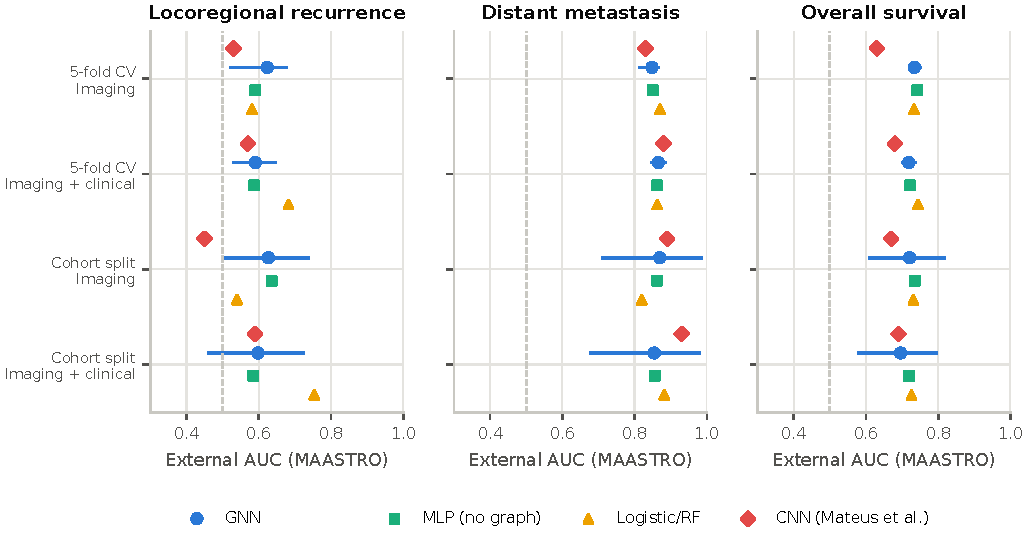
\includegraphics[width=0.92\textwidth]{Fig3.pdf}
\caption{External AUC on HN1 of the whole-tumour GNN (circles; CV: range of per-fold AUCs; cohort split: 95\% bootstrap CI) and of the MLP without edges (squares), both using whole-tumour features and selected on validation, compared with the published CNN (diamonds)~\cite{mateus2023}. The dashed line marks chance. CNN values from Mateus et al.~\cite{mateus2023}}\label{fig:auc}
\end{figure*}

\subsection{Tumour Definition Versus Tumour Burden}\label{sec:res-ablation}
The $2\times2$ ablation in Table~\ref{tab:ablation} and Fig.~\ref{fig:ablation} separates the two changes. With primary-GTV features, the GNNs outperformed the CNN in \winsPrimVol{} of 12 settings with volume bins and in \winsPrimBur{} of 12 with tumour-burden variables, and for DM they were 0.04 to 0.28 below the CNN in every setting. With whole-tumour features, the corresponding figures were \winsTotVol{} and \winsTotBur{} of 12.

Most of the improvement came from the tumour definition. Moving from the primary GTV to the whole tumour raised the DM AUC from \ablPrimVolDMMin--\ablPrimVolDMMax{} to \ablTotVolDMMin--\ablTotVolDMMax{} and the OS AUC from \ablPrimVolOSMin--\ablPrimVolOSMax{} to \ablTotVolOSMin--\ablTotVolOSMax, while LR hardly changed (\ablPrimVolLRMin--\ablPrimVolLRMax{} and \ablTotVolLRMin--\ablTotVolLRMax). Tumour-burden variables did help the primary-GTV models for DM when combined with imaging, raising the best value from \ablPrimVolDMMax{} to \ablPrimBurDMMax. Nodal burden clearly carries information about distant failure. Once the nodes were part of the radiomic region, however, the extra burden variables made no further difference.

% Table 4. Representation ablation (2 x 2): tumour region x clinical variables.
\begin{table*}[!tp]
\centering
\caption{Representation ablation: external AUC on HN1 of the GNN chosen on validation for each combination of radiomic tumour region and clinical variables. Values in bold exceed the CNN, whose values are taken from Mateus et al.~\cite{mateus2023}}\label{tab:ablation}
\tabsetup\setlength{\tabcolsep}{2.6pt}
\begin{tabularx}{\textwidth}{Q{3.0cm} Q{1.9cm} *{12}{C} P{1.0cm}}
\toprule
 & & \multicolumn{4}{c}{\tabh{LR (2 years)}} & \multicolumn{4}{c}{\tabh{DM (2 years)}} & \multicolumn{4}{c}{\tabh{OS (4 years)}} & \\
\cmidrule(lr){3-6}\cmidrule(lr){7-10}\cmidrule(lr){11-14}
 & & \multicolumn{2}{c}{\tabh{CV}} & \multicolumn{2}{c}{\tabh{Cohort}} & \multicolumn{2}{c}{\tabh{CV}} & \multicolumn{2}{c}{\tabh{Cohort}} & \multicolumn{2}{c}{\tabh{CV}} & \multicolumn{2}{c}{\tabh{Cohort}} & \\
\cmidrule(lr){3-4}\cmidrule(lr){5-6}\cmidrule(lr){7-8}\cmidrule(lr){9-10}\cmidrule(lr){11-12}\cmidrule(lr){13-14}
\tabh{Tumour region} & \tabh{Clinical} & \tabh{Img} & \tabh{+Cl} & \tabh{Img} & \tabh{+Cl} & \tabh{Img} & \tabh{+Cl} & \tabh{Img} & \tabh{+Cl} & \tabh{Img} & \tabh{+Cl} & \tabh{Img} & \tabh{+Cl} & \tabh{Wins}$^{a}$ \\
\midrule
\rowcolor{tabgroup}CNN$^{b}$ & -- & 0.53 & 0.57 & 0.45 & 0.59 & 0.83 & 0.88 & 0.89 & 0.93 & 0.63 & 0.68 & 0.67 & 0.69 & -- \\
Primary GTV & T, N, volume & \textbf{0.61} & \textbf{0.58} & \textbf{0.63} & \textbf{0.63} & 0.65 & 0.78 & 0.70 & 0.65 & \textbf{0.67} & \textbf{0.70} & 0.65 & 0.67 & 6/12 \\
Primary GTV & T, N, burden & \textbf{0.61} & \textbf{0.58} & \textbf{0.63} & \textbf{0.60} & 0.65 & 0.84 & 0.70 & 0.72 & \textbf{0.67} & \textbf{0.69} & 0.65 & \textbf{0.69} & 7/12 \\
Primary + nodal GTV & T, N, volume & \textbf{0.62} & \textbf{0.58} & \textbf{0.63} & \textbf{0.61} & \textbf{0.85} & 0.88 & 0.87 & 0.86 & \textbf{0.73} & \textbf{0.72} & \textbf{0.72} & \textbf{0.72} & 9/12 \\
Primary + nodal GTV & T, N, burden & \textbf{0.62} & \textbf{0.59} & \textbf{0.63} & \textbf{0.60} & \textbf{0.85} & 0.87 & 0.87 & 0.85 & \textbf{0.73} & \textbf{0.72} & \textbf{0.72} & \textbf{0.70} & 9/12 \\
\botrule
\end{tabularx}
\tabnote{CV: mean of the per-fold AUCs; Cohort: AUC in the cohort split. Img, imaging; +Cl, imaging and clinical; volume, GTV volume in four bins; burden, volume bins of the total GTV with the logarithm of the nodal GTV volume and the number of nodal GTV structures. $^{a}$Number of the 12 settings in which the GNN exceeded the CNN. $^{b}$Mateus et al.~\cite{mateus2023}, Tables 3 and 4.}
\end{table*}


\begin{figure*}[!tp]
\centering
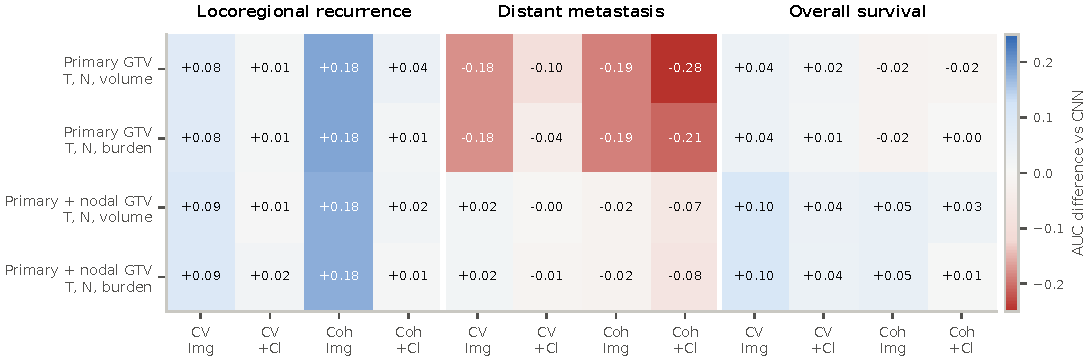
\includegraphics[width=0.92\textwidth]{Fig4.pdf}
\caption{Difference between the external AUC of the selected GNN and that of the CNN~\cite{mateus2023} for each combination of radiomic region (rows: primary GTV, or primary and nodal GTV) and clinical variables (volume bins or tumour burden), endpoint, design (CV; Coh, cohort split) and inputs (Img, imaging; +Cl, imaging and clinical). Blue: above the CNN; red: below. CNN values from Mateus et al.~\cite{mateus2023}}\label{fig:ablation}
\end{figure*}

\subsection{Contribution of the Patient-Similarity Graph}\label{sec:res-graph}
The MLP, which had the same node features and layers as the GNN but no edges, outperformed the CNN in \winsMLP{} of the 12 settings, one fewer than the GNNs (Table~\ref{tab:main}). The paired comparison in Table~\ref{tab:paired} shows that the external AUCs of the selected GNN and MLP differed by between \pairedDeltaMin{} and \pairedDeltaMax{} across the \pairedN{} endpoint, design and input combinations, including the clinical-only models. Only one difference reached nominal significance ($p=\pairedMinP$), and it favoured the MLP.

The matched comparison pointed the same way (Fig.~\ref{fig:matched}). Each of the \matchedN{} graph configurations was compared with the MLP that used exactly the same features. The GNN had the higher validation AUC in \matchedValFracAll\% of these pairs and the higher external AUC in \matchedTestFracAll\%, with a median external difference of \matchedTestMedAll. The graph did least harm for LR, where the GNN was better on HN1 in \matchedTestFracLR\% of pairs, and most harm for OS (\matchedTestFracOS\%). The advantage over the CNN came from the node features, and the edges did not add to it.

% Table 5. Paired comparison on HN1 of the GNN and the MLP without edges.
\begin{table*}[!tp]
\centering
\caption{Paired comparison on HN1 of the GNN and the MLP without edges, each chosen on validation with whole-tumour features}\label{tab:paired}
\tabsetup
\begin{tabularx}{\textwidth}{Q{2.0cm} Q{2.8cm} Q{2.0cm} P{1.6cm} P{1.6cm} C P{1.2cm}}
\toprule
\tabh{Design} & \tabh{Inputs} & \tabh{GNN model} & \tabh{GNN AUC} & \tabh{MLP AUC} & \tabh{$\Delta$AUC [95\% CI]}$^{a}$ & \tabh{$p$}$^{b}$ \\
\midrule
\grouprow{7}{Locoregional recurrence (2 years)}
5-fold CV & Imaging & GAT & 0.666 & 0.616 & +0.050 [$-$0.050, +0.150] & 0.38 \\
 & Imaging + clinical & GraphSAGE & 0.615 & 0.605 & +0.010 [$-$0.041, +0.066] & 0.72 \\
 & Clinical & GCN & 0.576 & 0.570 & +0.006 [$-$0.019, +0.032] & 0.65 \\
Cohort split & Imaging & GCN & 0.627 & 0.636 & $-$0.009 [$-$0.045, +0.027] & 0.63 \\
 & Imaging + clinical & GCN & 0.598 & 0.585 & +0.013 [$-$0.024, +0.053] & 0.52 \\
 & Clinical & GAT & 0.507 & 0.478 & +0.029 [$-$0.011, +0.069] & 0.17 \\
\grouprow{7}{Distant metastasis (2 years)}
5-fold CV & Imaging & GCN & 0.882 & 0.878 & +0.004 [$-$0.009, +0.022] & 0.72 \\
 & Imaging + clinical & GraphSAGE & 0.867 & 0.873 & $-$0.006 [$-$0.028, +0.013] & 0.66 \\
 & Clinical & GAT & 0.829 & 0.843 & $-$0.014 [$-$0.051, +0.013] & 0.38 \\
Cohort split & Imaging & GraphSAGE & 0.870 & 0.861 & +0.008 [$-$0.014, +0.033] & 0.51 \\
 & Imaging + clinical & GCN & 0.854 & 0.856 & $-$0.001 [$-$0.031, +0.031] & 0.91 \\
 & Clinical & GCN & 0.793 & 0.814 & $-$0.021 [$-$0.063, +0.012] & 0.28 \\
\grouprow{7}{Overall survival (4 years)}
5-fold CV & Imaging & GCN & 0.741 & 0.744 & $-$0.004 [$-$0.018, +0.011] & 0.64 \\
 & Imaging + clinical & GCN & 0.720 & 0.723 & $-$0.003 [$-$0.017, +0.012] & 0.72 \\
 & Clinical & GAT & 0.692 & 0.715 & $-$0.023 [$-$0.047, $-$0.001] & 0.03$^{*}$ \\
Cohort split & Imaging & GraphSAGE & 0.721 & 0.735 & $-$0.014 [$-$0.051, +0.021] & 0.38 \\
 & Imaging + clinical & GraphSAGE & 0.696 & 0.719 & $-$0.023 [$-$0.055, +0.005] & 0.13 \\
 & Clinical & GCN & 0.701 & 0.704 & $-$0.003 [$-$0.029, +0.023] & 0.79 \\
\botrule
\end{tabularx}
\tabnote{In CV, the predictions of the five fold models were averaged before the AUC was computed. $^{a}$GNN minus MLP, with 95\% paired patient-level bootstrap CI (2000 resamples). $^{b}$Two-sided bootstrap $p$ value. $^{*}p<0.05$.}
\end{table*}


\begin{figure*}[!tp]
\centering
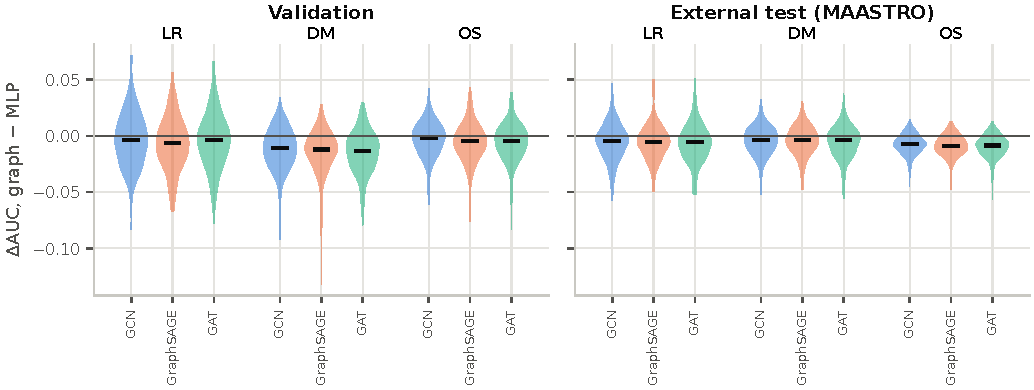
\includegraphics[width=0.92\textwidth]{Fig5.pdf}
\caption{Matched comparison of every graph configuration with the MLP using identical features (feature set, selector, subset size and inputs), on validation (left) and on HN1 (right), by endpoint and GNN architecture. Values above zero favour the graph. Horizontal lines inside the violins mark medians}\label{fig:matched}
\end{figure*}

\subsection{Training Randomness and Conventional Classifiers}\label{sec:res-seed}
Retraining each selected configuration with \seedRepeats{} non-overlapping ten-seed ensembles changed the external AUC very little. The standard deviation (SD) across re-runs had a median of \seedSDmed{} and a maximum of \seedSDmax{} (Fig.~\ref{fig:seed}, Table S2 in Online Resource~1). The GNN beat the CNN in every re-run in \seedStableWins{} of the 12 settings and in none of the re-runs in the other \seedStableLoss. The comparison with the CNN did not depend on the seeds chosen for the reported models.

Conventional classifiers trained on the same whole-tumour features with the extended clinical set reached external AUCs of \clsLRMin--\clsLRMax{} for LR, \clsDMMin--\clsDMMax{} for DM and \clsOSMin--\clsOSMax{} for OS, and they too outperformed the CNN in \winsCls{} of the 12 settings (Table~\ref{tab:main}). With imaging alone, they performed similarly to the GNNs for DM and OS and worse for LR. With clinical data added, they reached \clsLRCVClin{} and \clsLRCohClin{} for LR, well above the GNNs. The clinical variables, not the radiomic features, accounted for this difference. Logistic regression on these clinical variables alone, which include age, HPV status and tumour subsite as well as T and N category, reached \clsClinLRMin--\clsClinLRMax{} for LR, \clsClinDMMin--\clsClinDMMax{} for DM and \clsClinOSMin--\clsClinOSMax{} for OS. In the cohort split for LR, the model selected with clinical inputs was in fact the clinical model with GTV volume and no texture features. The GNNs used only the clinical variables of the CNN study, which include neither age nor HPV status.

\begin{figure*}[!tp]
\centering
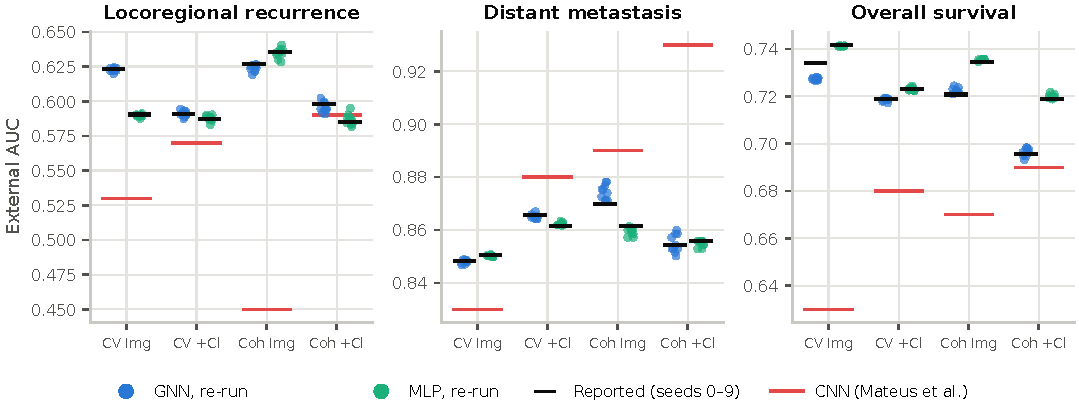
\includegraphics[width=0.92\textwidth]{Fig6.pdf}
\caption{External AUC on HN1 of the selected GNNs (blue) and MLPs (green) after retraining with non-overlapping ten-seed ensembles, by endpoint, design (CV; Coh, cohort split) and inputs (Img, imaging; +Cl, imaging and clinical). Black bars: reported models (seeds 0--9); red lines: CNN~\cite{mateus2023}}\label{fig:seed}
\end{figure*}

%% =========================================================================================
\section{Discussion}\label{sec:discussion}
On the public protocol of Mateus et al., GNNs built on radiomic features of the whole tumour matched or exceeded the published CNN for LR and OS and came close to it for DM. The same networks built on the primary GTV fell well short for DM. The ablation traced this gap to the tumour definition rather than to tumour burden entered as a clinical variable. The no-edge comparison showed that the patient-similarity graph itself contributed nothing measurable. The MLP reached the same external discrimination, the paired differences were small and went in both directions, and with identical features the GNN was worse more often than it was better.

Why should the tumour definition matter so much? Two explanations fit the data. The first is biological. Nodal disease and total tumour volume are among the strongest predictors of distant metastasis in HNSCC~\cite{kjems2023volume,jensen2020nodalfdg}. A radiomic description of the primary tumour cannot capture them, whereas the CNN, which saw the whole image, could. The second is a measurement problem. Separate nodal GTVs were drawn in \nodalPctCan\% of HN-PET-CT patients but \nodalPctMAA\% of HN1 patients, and at one Canadian centre nodal disease seems to have been included in the structure labelled as the primary GTV. A model trained on the primary GTV thus learnt from a structure that sometimes contained nodes and was tested on one that usually did not, and part of its DM signal could not transfer. Using the union of all GTVs removes this mismatch, because the whole delineated tumour is described the same way however it was subdivided. These data cannot fully separate the two explanations. Both, however, point to the same practical advice. Radiomic models compared with image-based deep learning should use the tumour region that the network sees, and delineation conventions in public cohorts should be checked before features are compared across them.

The negative result for the graph is consistent with earlier work on patient-similarity graphs. The gains reported in neuroimaging and COVID-19 pneumonia were obtained with richer non-imaging data defining the edges, and they were seldom tested against an equally tuned network without edges~\cite{parisot2018population,keicher2023covid}. In this study, the edges were defined by the same features as the nodes. Message passing could only pull each patient's prediction towards those of similar training patients, which an MLP on the same features can largely reproduce. With a few hundred patients and a handful of selected features, this smoothing adds no information that the features do not already hold. Without the no-edge control, the conclusion would have been different: the GNNs did outperform the CNN in \winsGraph{} of 12 settings, and on its own this result could easily have been credited to the graph. Studies of graph-based outcome models should therefore routinely report the same network trained without edges.

The conventional classifiers support this reading. On the same whole-tumour features, logistic regression and random forests matched the GNNs, which again places the gain in the features. For LR, a fuller clinical description that included age and HPV status outperformed every imaging model and the CNN. The comparison with the CNN was intentionally limited to the clinical variables the CNN had used, so that both approaches received the same information. It should not be taken to mean that imaging adds to a complete clinical model for LR, and these data do not suggest that it does. Training randomness did not change any of these conclusions. Every configuration was a ten-seed ensemble, and re-runs with fresh seeds varied by a few thousandths of an AUC at most. For CT radiomics in HNSCC cohorts of this size, what is measured appears to matter more than the architecture used to combine the measurements.

This study has several limitations. The whole-tumour representation was introduced after the primary-GTV results had been seen, so the HN1 data were used more than once. This risk was reduced by the prior rationale (the CNN input contains the nodes), by selecting every model on validation data and by reporting all four ablation representations, but the whole-tumour results still need confirmation in an independent cohort. The DM test set had only \eTestDM{} events, which makes the DM AUCs imprecise and leaves differences of a few hundredths unresolved. The comparison with the CNN is descriptive, because its predictions are not available for a paired test. Nodal delineations in public collections are incomplete and their conventions are not documented, so the whole tumour as defined here depends on what each centre chose to contour. Calibration, clinical utility and performance in sociodemographic subgroups were not assessed. The aim was to compare discrimination with a CNN for which only AUCs were reported, but a model intended for clinical use would need these analyses. Finally, only CT radiomics was studied, and graphs whose edges are built from other data, such as genomics or PET, may behave differently.

In conclusion, on the public benchmark protocol of a published CNN, the external discrimination of radiomic GNNs in HNSCC was determined by the tumour region that the features described and not by the patient-similarity graph. Describing the primary and nodal GTVs together allowed these networks to match or exceed the CNN for locoregional recurrence and overall survival and to approach it for distant metastasis, whereas the graph added nothing over the same network without edges, and for locoregional recurrence a clinical model that included HPV status remained stronger than any imaging model. Radiomic studies compared with image-based networks should describe the same tumour region, imaging models should be compared with a complete clinical model, and graph-based outcome models should be reported together with their edgeless counterpart.

%% =========================================================================================
\bmhead{Supplementary Information}
The online version contains supplementary material in Online Resource~1 (ESM\_1.pdf). Table S1 lists the configurations selected on validation, Table S2 gives the results of the seed re-runs, and Tables S3--S7 contain the completed TRIPOD+AI, CLAIM 2024, CLEAR, METRICS and RQS checklists.

\bmhead{Acknowledgements}
The author thanks the investigators who made the Head-Neck-PET-CT and HN1 collections publicly available through The Cancer Imaging Archive.

\section*{Statements and Declarations}

\bmhead{Funding}
No funding was received for conducting this study.

\bmhead{Competing Interests}
The author has no relevant financial or non-financial interests to disclose.

\bmhead{Author Contributions}
Conceptualization, methodology, software, formal analysis, investigation, data curation, visualization, writing (original draft) and writing (review and editing): Hasan Shaikh. The author read and approved the final manuscript.

\bmhead{Data Availability}
All data analysed in this study are publicly accessible. The CT images, radiotherapy structure sets and clinical data of the development cohort are available from The Cancer Imaging Archive as the Head-Neck-PET-CT collection (\url{https://doi.org/10.7937/K9/TCIA.2017.8oje5q00}) and those of the external test cohort as the HN1 collection (\url{https://doi.org/10.7937/tcia.2019.8kap372n}), under the data usage policies of The Cancer Imaging Archive. No new patient data were generated. The radiomic features, tumour volumes and predictions derived in this study can be regenerated from these collections with the released code. The performance of the CNN was taken from the published report of Mateus et al.~\cite{mateus2023}.

\bmhead{Code Availability}
The code for feature extraction, construction of the patient-similarity graphs, model training and selection, the ablation and seed analyses, and the script that generates every table, figure and quoted number of this manuscript is openly available at \url{https://github.com/hash123shaikh/Radiomics_Graph_Attention_Network_HNC} under the MIT licence, together with the software environment and step-by-step instructions to reproduce the results.

\section*{Compliance with Ethical Standards}

\bmhead{Disclosure of Potential Conflicts of Interest}
The author declares that there are no conflicts of interest.

\bmhead{Research Involving Human Participants and/or Animals}
This study is a secondary analysis of de-identified, publicly available data from The Cancer Imaging Archive; no new data were collected from human participants and no animals were involved. The original studies that created the collections obtained institutional ethics approval, and separate ethics approval was therefore not required for this analysis.

\bmhead{Informed Consent}
Not applicable to this secondary analysis. Informed consent, or a waiver of consent, was obtained by the original studies under their institutional approvals.

\bibliography{references}

\end{document}
